\documentclass{article}

\usepackage[utf8]{inputenc}
\usepackage{graphicx}
\graphicspath{ {Project2/figures/} }
\usepackage{float}
\usepackage{listings}
\usepackage{amsmath}
\usepackage{amssymb}
\usepackage{mathtools}
\usepackage{commath}
\usepackage{tabularx}
\usepackage[ruled,vlined]{algorithm2e}
\usepackage{caption}
% \usepackage{subcaption}
\usepackage[outputdir=../]{minted}
\usepackage{verbatim}
\usepackage{tikz}
\usepackage{bm}

\usepackage{comment}
\usepackage[style=apa]{biblatex}
\addbibresource{Project2/refs.bib}

\usepackage{subfig}

\usepackage{amsthm}
\usepackage{enumitem}
\usepackage{breakcites}

\newtheorem{theorem}{Theorem}[section]
\newtheorem{lemma}[theorem]{Lemma}
\theoremstyle{definition}
\newtheorem{definition}{Definition}[subsection]


% \bibliographystyle{apalike}
\usepackage{hyperref}
\hypersetup{breaklinks=true,colorlinks=true,linkcolor=blue,citecolor=blue,filecolor=magenta,urlcolor=blue}

\DeclareMathOperator*{\argmax}{arg\,max}
\DeclareMathOperator*{\argmin}{arg\,min}
\DeclareMathOperator*{\sgn}{sgn}
\DeclareMathOperator*{\Bias}{Bias}
\DeclareMathOperator*{\Var}{Var}


\title{Classification and Regression}
\author{Femtehjell, Hoel, Otterlei and Steeneveldt}

\date{October 2023}


% \def\@bibdataout@aps{%
% \immediate\write\@bibdataout{%
% @CONTROL{%
% apsrev41Control%
% \longbibliography@sw{%
%     ,author="08",editor="1",pages="1",title="0",year="1"%
%     }{%
%     ,author="08",editor="1",pages="1",title="",year="1"%
%     }%
%   }%
% }%
% \if@filesw \immediate \write \@auxout {\string \citation {apsrev41Control}}\fi
% }

\begin{document}

\setminted[python]{frame=lines,
    framesep=2mm,
    linenos,
    fontsize=\footnotesize,
    mathescape=true,
    escapeinside=||
}

\maketitle
\begin{figure}[H]
    \centering
    
\includegraphics[scale=0.5]{1797261_uio-logo.png}
\end{figure}
\newpage
\tableofcontents
\listoffigures


\newpage

\begin{abstract}
    The abstract will go here
\end{abstract}

\section{Introduction}
The idea of artificial intelligence is an old idea stretching back to the greeks of the late antiquity. "Automaton" is the word they used. A machine that could operate itself. The idea has kept fascinating humanity over the centuries, to Leonardo DaVinci and his mechanical knight, to "The turk" in the 18th century and to the modern area. In the 1940's, Warren McCullouch and Walter Pitts came up with a mathematical model to describe the neuron cell in the brain. They called this model threshold logic \textbf{(legg til kilde)}. Later, this model has inspired and evolved into what we call neural networks. Networks of cells made to mimick the brain and simulated on a computer to learn complex tasks it can solve on its own. \\
In scientific research, the use of neural networks has exploded and the set of variations on different architectures keeps expanding. FFNN is the biggest category of artificial neural network (ANN) and other types of ANNs, such as recurrent neural networks, even builds upon it. This naturally makes it interesting to see how one can build a good FFNN model. \\
The key part to a good neural network is optimization. As a neural network consists of layers upon layers of neurons connected to each other (as will be explained later), optimizing all the computations 
This project will first take a look at the theory behind neural network. Starting with a theoretical aspect of optimization and moving to the theoretical models of feed forward neural network and logistic regression. Then moving on to the methods used in the project to test different techniques, as well as the results from these techniques. Further, the results will be discussed and lastly a conclusion of the project will be (something, cant find the word).

\newpage

\section{Theory}

\subsection{The Cost function}
In machine learning, the primary goal is to make accurate predictions based on known input data. The nature of these predictions can vary widely depending on the task at hand. For instance, a machine learning algorithm may predict whether an email is spam or not, an application of binary classification. In other cases, the algorithm might be used to anticipate the price of a house given certain features like its size, location and age, illustrating a regression task.

Alternatively, it could predict whether a given image depicts a cat, a dog, a horse, or some other animal, a scenario referred to as multi-class classification. Similarly, algorithms can also forecast sequences of data, such as the words that come next in a sentence, generally considered as sequence prediction problems. In all these scenarios, the machine learning model uses patterns recognized from training data to make these predictions. The measure of accuracy from these predictions subsequently determines the subsequent course of action, i.e., optimizing the model's performance, which is where the concept of a cost function comes in


The cost function serves as a measure for a model's performance on a specific data set. It is what defines the multidimensional 'cost surface' we wish to minimize with respect to our model parameters. The choice of cost function is thus very important. The optimal cost function is dependent on the specific task at hand – whether it be regression, binary classification, or multi-class classification.

During regression analysis, where the aim is to predict a single response variable based on one or more independent variables. We assume our observed response (y) can be modeled as

\begin{equation*}
    y = f(\mathbf{x}) + \epsilon
\end{equation*}
$\mathbf{x}$ are our dependent variables and $\epsilon$ is 
the stochastic noise inherent in $y$. We may assume $\epsilon \sim N(0,\sigma^2)$.
We consider $n$ samples of $y$ and assume that there are $p$ characteristics which define each of the samples, such that $y_i = f(\boldsymbol{x}_i) + \varepsilon_i$ where $\boldsymbol{x}_i = \left[x_{i,0}, x_{i, 1}, \ldots, x_{i, p-1} \right]$.

We gather this information in a matrix $\textbf{X}$, called the design matrix, such that
\begin{equation*}
    \textbf{X} =
    \begin{bmatrix}
        x_{0,0} & x_{0,1} & \ldots & x_{0, p-1} \\
        x_{1,0} & x_{1,1} & \ldots & x_{1, p-1} \\
        \vdots & \vdots & \ddots & \vdots \\
        x_{n,0} & x_{n,1} & \ldots & x_{n, p-1}
    \end{bmatrix}.
\end{equation*}


It is common practice to use Mean Squared Error (MSE). Additionally, to avoid overfitting and improve generalization, we often include a $L1$ or $L2$ regularization term in the cost function. 

\begin{align*}
C_{LS} (\boldsymbol{\theta}(\mathbf{X})) =& \frac{1}{n} \sum_{i=1}^{n-1}\left(y_i - \boldsymbol{\theta}(\boldsymbol{x_i})\right)^2\\[1mm]
C_{L-1} (\boldsymbol{\theta}(\mathbf{X}))= & \hspace{1mm} C_{LS}(\boldsymbol{\theta}(\mathbf{X})) + \lambda ||\boldsymbol{\theta}||_1\\[3mm]
C_{L-2} (\boldsymbol{\theta}(\mathbf{X}))= & \hspace{1mm} C_{LS}(\boldsymbol{\theta}(\mathbf{X})) + \lambda  ||\boldsymbol{\theta}||_2
\end{align*}

Here $\boldsymbol{\theta}$ denotes the parameters/weights of the network,  $\boldsymbol{X}$  the input data,  $\lambda$ the strength of the regularization and the subscript $LS$ denotes least squares. If our model is predicting a vector MSE might be used as a loss function instead.

\begin{align*}
C (\boldsymbol{\theta}(\mathbf{X})) =& \frac{1}{n} \sum_{i=1}^{n-1} \frac{1}{m}\sum_{j=1}^{m-1} \left(y_{i,j} - \boldsymbol{\theta}(\boldsymbol{x_i})\right)^2 =  \frac{1}{n} \sum_{i=1}^{n-1} MSE(\boldsymbol{y}_i - \boldsymbol{\theta(x_i)}) \\[1mm]
C_{L-1} (\boldsymbol{\theta}(\mathbf{X}))= & \hspace{1mm} C(\boldsymbol{\theta}(\mathbf{X})) + \lambda ||\boldsymbol{\theta}||_1\\[3mm]
C_{L-2} (\boldsymbol{\theta}(\mathbf{X}))= & \hspace{1mm} C(\boldsymbol{\theta}(\mathbf{X})) + \lambda  ||\boldsymbol{\theta}||_2
\end{align*}



\subsubsection{OLS and Ridge}
Whenever $\boldsymbol{\theta}$ is a linear function we recover ordinary least squares.

The linear relationship we are assuming is such that $y_i = \mathbf{x}_i \cdot \bm{\beta} + \epsilon$. We can write this more compact as
\begin{equation*}
    \mathbf{y} =
    \begin{bmatrix}
        x_{0,0} & x_{0,1} & \ldots & x_{0, p-1} \\
        x_{1,0} & x_{1,1} & \ldots & x_{1, p-1} \\
        \vdots & \vdots & \ddots & \vdots \\
        x_{n,0} & x_{n,1} & \ldots & x_{n, p-1}
    \end{bmatrix}
    \begin{bmatrix}
        \beta_0 \\
        \beta_1 \\
        \vdots \\
        \beta_{p-1}
    \end{bmatrix}
    +
    \begin{bmatrix}
        \epsilon_0 \\
        \epsilon_1 \\
        \vdots \\
        \epsilon_{p-1}
    \end{bmatrix}
    = \mathbf{X}\bm{\beta} + \epsilon
\end{equation*}
where the $\mathbf{X}$ is called the design matrix and $\bm{\beta}$ is called weights. Our optimal OLS model is thus given by
\begin{equation*}
    \bm{\hat{\beta}} = \argmin_{\beta \in \mathbb{R}^p}\tfrac{1}{n}(\mathbf{y} - \mathbf{X}\bm{\beta})^T(\mathbf{y} - \mathbf{X}\bm{\beta})
\end{equation*}

If we add our $L2$ regularization term we get ridge regression. We then wish to minimize
\begin{equation*}
    \bm{\hat{\beta}} = \argmin_{\beta \in \mathbb{R}^p}\tfrac{1}{n}(\mathbf{y} - \mathbf{X}\bm{\beta})^T(\mathbf{y} - \mathbf{X}\bm{\beta}) + \lambda\bm{\beta}^2
\end{equation*}

\subsubsection{Binary Classification}
When we use MSE as a loss function, we're primarily asking the model, "How far is your prediction from the actual value?" This question is appropriate in regression, where we're predicting values on a continuous scale. However, in classification, we are more interested in getting the class label right, i.e., whether a prediction falls into class 0 or class 1, rather than exactly how far the predicted probability is from the actual value of 0 or 1.

Let's consider a binary classification problem and we have an example that belongs to class 1, but our model predicts it as class 0. So it's a complete misclassification, the square loss however is only 1! Instead of MSE we may use binary cross entropy (BCE).

 To find the BCE loss we evaluate the distance between our predicted probability value (p) and the actual value (which could be either y=0 or y=1). The loss function is given by

\[
L(y, p) = -ylog(p) - (1-y)log(1-p)
\]
If $y=1$ then
\[
L(y,p) = -log(p)
\]
Clearly  $L \to 0$ as $p \to 1$ and $L \to \infty$ as $p \to 0$
if $y = 0$ then
\[
L(y,p) = -log(1-p)
\]
Here $L \to 0$ as $p \to 0$ and $L \to \infty$ as $p \to 1$
The loss is thus much more appropriate.


The BCE cost function is simply mean of $n$ such losses.

\[
C(\mathbf{y}, \mathbf{p}) = \frac{1}{n} \sum_{i=1}^{n} L(y_i, p_i)
\]

Minimizing this is the purpose of a binary classifier

\subsubsection{Logistic Regression}
%In classification problems, the variables are discrete (i.e. categories). As an example, in medicine, one might want to predict if someone has had a stroke or not given certain medical signs. Thus we have two categories, $\{\text{'Stroke'}, \text{'No\ stroke'}\}$ or simply $\{1,0\}$. 
Logistic regression is a method for obtaining a binary classifier where we assume a linear relationship between the input features and the binary category.


We assume that the probability of features 
$\mathbf{x}_i = \left[x_{i,0}, x_{i, 1}, \ldots, x_{i, p-1} \right]$ land us in category $\mathbf{y}$ ($0$ or $1$)is best modeled by

\begin{equation*}
f(\mathbf{x_i}\bm{\beta})
\end{equation*}

Where $f: \mathbb{R} \to (0,1)$. This ensures a valid probability for the predicted values. For logistic regression we use the logistic function, also known as the sigmoid function 
\begin{equation*}
    \sigma(z) = \frac{1}{1 + e^{-z}} = \frac{e^{z}}{1 + e^z}
\end{equation*}
We thus get for our prediction
\begin{equation*}
    p(\mathbf{x}_i) = \frac{e^{\mathbf{x}_i\bm{\beta}}}{1 + e^{\mathbf{x}_i\bm{\beta}}}
\end{equation*}
When the logarithm is taken, it reveals the linear relationship once more
\begin{equation*}
    \log(p(\mathbf{x}_i)) = \mathbf{x}_i\bm{\beta}
\end{equation*}
To fit this model we find the $\bm{\beta}$ which maximises the likelihood function
\begin{equation*}
    L(\bm{\beta}) = \prod_{i: y_i = 1}p(x_i)\prod_{j:y_j = 0}(1-p(x_j))
\end{equation*}
which we can write as
\begin{equation*}
    L(\bm{\beta}) = \prod_{i=1}^{n}P(y_i | \mathbf{x}_i,\bm{\beta})
\end{equation*}
where $n$ is the number of samples and $P(y_i | \mathbf{x}_i,\bm{\beta})$ is the probability of $y_i$ given the input $\mathbf{x}_i$ and the weights $\bm{\beta}$. Maximizing this equation is what we call the method of maximum likelihood. To simplify, we take the log of the equation and get the log-likelihood and also multiply with $-1$ such that it becomes a minimization problem instead of a maximization problem
\begin{equation*}
    \begin{split}
        \ell(\bm{\beta}) & = -\sum_{i=1}^{n}(y_i\log(p(\mathbf{x}_i) + (1 - y_i)\log(1 - p(\mathbf{x}_i)) \\
        & = -\sum_{i=1}^{n}(y_i\log(p(\mathbf{x}_i) + \log(1 - p(\mathbf{x}_i)) - y_i\log(1 - p(\mathbf{x}_i)) \\
        & = -\sum_{i=1}^{n}(y_i\mathbf{x}_i\bm{\beta} + \log(1 - p(\mathbf{x}_i)))
    \end{split}
\end{equation*}
 This is just the binary cross entropy cost without $\frac{1}{n}$. The same cost function used for binary classification, even when there is not a linear relationship between the features and the observed categories. 
 To minimize, we differentiate with respect to $\bm{\beta}$. First, the derivative of the sigmoid function is
\begin{equation*}
    \frac{\partial \sigma(z)}{\partial z} = \sigma(z) - \sigma(z)^2 = \sigma(z)(1 - \sigma(z))
\end{equation*}

\begin{comment}
\subsubsection{Binary classification}

When we use MSE as a loss function, we're primarily asking the model, "How far is your prediction from the actual value?" This question is appropriate in regression, where we're predicting values on a continuous scale. However, in classification, we are more interested in getting the class label right, i.e., whether a prediction falls into class 0 or class 1, rather than exactly how far the predicted probability is from the actual value of 0 or 1.

Let's consider a binary classification problem:

Case 1) Suppose we have an example that belongs to class 1, but our model predicts it as class 0. So it's a complete misclassification. Case 2) A different data point also belongs to class 1, and this time, the model predicts 0.9, which is quite close to the actual value and is indeed predicting the correct class (as 0.9 is closer to 1).

In both these cases, by focusing only on the MSE, we are more concerned with the difference between the predicted and actual values, not taking into account the notion of 'correctly classified' or 'misclassified'. For these reasons the binary cross entropy (BCE) is preferred.

Binary Cross Entropy (BCE), we evaluate the distance between our predicted probability value (p) and the actual value (which could be either y=0 or y=1). The loss function is given by

\[
L(y, p) = -ylog(p) - (1-y)log(1-p)
\]
If $y=1$ then
\[
L(y,p) = -log(p)
\]
Clearly  $L \to 0$ as $p \to 1$ and $L \to \infty$ as $p \to 0$
if $y = 0$ then
\[
L(y,p) = -log(1-p)
\]
Here $L \to 0$ as $p \to 0$ and $L \to \infty$ as $p \to 1$

The BCE cost function is simply mean of $n$ such losses.

\[
C(\mathbf{y}, \mathbf{p}) = \frac{1}{n} \sum_{i=1}^{n} L(y_i, p_i)
\]
\end{comment}

\begin{comment}
\subsection{Regression}

\subsubsection{OLS}

%Ordinary least squares is a method used to best fit a line to a set of data points. It minimizes the sum of squared residuals, which means it finds the distance between the input data points and the points along the line. The goal is to find the best relationship between a independent variable $\mathbf{x}$ (the input data) and a dependent variable $\mathbf{y}$ (the observed data).
%Assume there exists some functional relationship between a set of variables $\mathbf{x}$ and a single stochastic variable $y$. We may denote these as explanatory and response variables. 

Ordinary least squares is a method used to best fit a line to a set of data points. It minimizes the sum of squared residuals, which means it finds the distance between the input data points and the points along the line. The goal is to find the best relationship between a independent variable $\mathbf{x}$ (the input data) and a dependent variable $\mathbf{y}$ (the observed data).

\begin{equation*}
    y = f(\mathbf{x}) + \epsilon
\end{equation*}

$\epsilon$ is 
the stochastic noise inherent in $y$. We may assume $\epsilon \sim N(0,\sigma^2)$.
For example one could denote $y$ as being the number of beach goers and our explanatory variables could be the temperature, the wind speed, the time of the day, the number of ice cream flavours available and so on.

 We are then looking for an approximation of $f$ which gives $\tilde{\boldsymbol{y}}$ such that the MSE, $\frac{1}{n} \left( \boldsymbol{y} - \tilde{\boldsymbol{y}} \right)^2$, is minimized. In order to approximate $f$, we consider $n$ samples of $\boldsymbol{y}$ and assume that there are $p$ characteristics which define each of the samples, such that $y_i = f(\boldsymbol{x}_i) + \varepsilon_i$ where $\boldsymbol{x}_i = \left[x_{i,0}, x_{i, 1}, \ldots, x_{i, p-1} \right]$.

We gather this information in a matrix $\textbf{X}$, called the design matrix, such that
\begin{equation*}
    \textbf{X} =
    \begin{bmatrix}
        x_{0,0} & x_{0,1} & \ldots & x_{0, p-1} \\
        x_{1,0} & x_{1,1} & \ldots & x_{1, p-1} \\
        \vdots & \vdots & \ddots & \vdots \\
        x_{n,0} & x_{n,1} & \ldots & x_{n, p-1}
    \end{bmatrix}.
\end{equation*}

where $\mathbf{y} \in Y$ is our observed data, $\mathbf{x} \in X$ is the input data and $\epsilon$ is the error term given as $\epsilon \sim N(0,\sigma^2)$. Looking to approximate $f$, we consider $n$ samples and assume that there are $p$ characteristics which define each of the samples, such that $y_i = f(\mathbf{x}_i) + \epsilon_i$, with $\mathbf{x}_i = [x_{i,0},x_{i,1},...,x_{i,p-1}]$. The approximation of $f$ should give us $\mathbf{\Tilde{y}}$ such that $\tfrac{1}{n}(\mathbf{y} - \mathbf{\Tilde{y}})$ is minimized. \\
... \\
We assume a linear relationship such that $y_i = \mathbf{x}_i \cdot \bm{\beta} + \epsilon$. We can write this more compact as
\begin{equation*}
    \mathbf{y} =
    \begin{bmatrix}
        x_{0,0} & x_{0,1} & \ldots & x_{0, p-1} \\
        x_{1,0} & x_{1,1} & \ldots & x_{1, p-1} \\
        \vdots & \vdots & \ddots & \vdots \\
        x_{n,0} & x_{n,1} & \ldots & x_{n, p-1}
    \end{bmatrix}
    \begin{bmatrix}
        \beta_0 \\
        \beta_1 \\
        \vdots \\
        \beta_{p-1}
    \end{bmatrix}
    +
    \begin{bmatrix}
        \epsilon_0 \\
        \epsilon_1 \\
        \vdots \\
        \epsilon_{p-1}
    \end{bmatrix}
    = \mathbf{X}\bm{\beta} + \epsilon
\end{equation*}
where the $\mathbf{X}$ is called the design matrix and $\bm{\beta}$ is called weights. Wanting to find
\begin{equation*}
    \bm{\hat{\beta}} = \argmin_{\beta \in \mathbb{R}^p}\tfrac{1}{n}(\mathbf{y} - \mathbf{X}\bm{\beta})^T(\mathbf{y} - \mathbf{X}\bm{\beta})
\end{equation*}
and knowing that
\begin{equation*}
    (\mathbf{y} - \mathbf{X}\bm{\beta})^T(\mathbf{y} - \mathbf{X}\bm{\beta}) = \mathbf{y}^T\mathbf{y} - 2\bm{\beta}^T\mathbf{X}^T\mathbf{y} + \bm{\beta}^T\mathbf{X}^T\mathbf{X}\bm{\beta}
\end{equation*}
we can compute the partial derivatives of the above expression and neglect the scaling factor $\tfrac{1}{n}$. This gives us
\begin{gather*}
    \frac{\partial}{\partial \boldsymbol{\beta}} \left( \boldsymbol{y}^T \boldsymbol{y} - 2 \boldsymbol{\beta}^T \textbf{X}^T \boldsymbol{y} + \boldsymbol{\beta}^T \textbf{X}^T \textbf{X} \boldsymbol{\beta} \right) = 0 \\
    -2 \textbf{X}^T \boldsymbol{y} + 2 \textbf{X}^T \boldsymbol{X \beta} = 0 \\
    2 \textbf{X}^T \boldsymbol{X \beta} = 2 \textbf{X}^T \boldsymbol{y} \\
    \boldsymbol{\beta} = \left( \textbf{X}^T \textbf{X} \right)^{-1} \textbf{X}^T \boldsymbol{y}
\end{gather*}
Now we have an analytical expression for the weights, which is what we wanted.
For a more detailed and longer explanation of OLS, including the expectation and variance of OLS, see (project 1 link goes here)

\subsubsection{Ridge}
Overfitting is the concept where the model learns the training data too well, and failing to generalize to other data sets. As an analogy, this would be similar to someone learning what numbered answer to answer on a test instead of actually learning the topic of the test. This can be a challenge in OLS and thus we introduce a regularization term in ridge regression. The new expression to minimize becomes
\begin{equation*}
    \bm{\hat{\beta}} = \argmin_{\beta \in \mathbb{R}^p}\tfrac{1}{n}(\mathbf{y} - \mathbf{X}\bm{\beta})^T(\mathbf{y} - \mathbf{X}\bm{\beta}) + \lambda\bm{\beta}^2
\end{equation*}
where the right hand side multiplies to
\begin{equation*}
    \frac{1}{n}(\mathbf{y}^T\mathbf{y} - 2\bm{\beta}^T\mathbf{X}^T\mathbf{y} + \bm{\beta}^T\mathbf{X}^T\mathbf{X}\bm{\beta}) + \lambda\bm{\beta}^T\bm{\beta}
\end{equation*}
Finding again the partial derivatives, we get
\begin{gather*}
    \frac{\partial}{\partial \boldsymbol{\beta}} \left( \left( \boldsymbol{y} - \textbf{X} \boldsymbol{\beta} \right)^2 + \lambda \boldsymbol{\beta}^2 \right) = 0 \\
    -2 \textbf{X}^T \boldsymbol{y} + 2 \textbf{X}^T \boldsymbol{X \beta} + 2\lambda \boldsymbol{\beta} = 0 \\
    \textbf{X}^T \boldsymbol{X \beta} + \lambda \boldsymbol{\beta} = \textbf{X}^T \boldsymbol{y} \\
    \left(\textbf{X}^T \textbf{X} + \boldsymbol{I}_p \lambda \right) \boldsymbol{\beta} = \textbf{X}^T \boldsymbol{y} \\
    \boldsymbol{\beta} = \left(\textbf{X}^T \textbf{X} + \boldsymbol{I}_p \lambda \right)^{-1} \textbf{X}^T \boldsymbol{y}
\end{gather*}
For a more detailed explanation of ridge regression, see (Project 1 link)
\end{comment}




\subsection{Optimization}

%%At the core of most issues within machine learning and data analysis, we find an optimization problem.  In a perfect scenario we would like to like to find this analytically, however for various reasons, whether they be computational or purely mathematical in nature, this is often not possible. 
As we've observed, the cost function is at the core of solving machine learning problems, which fundamentally involve optimization. That is we wish to find the minimum of a function. In a perfect scenario we would like to find this analytically, however for various reasons, whether they be computational or purely mathematical in nature, this is often not possible. Therefore we opt for iterative methods instead.
\subsubsection{Gradient descent}

Let  $$f: \mathbf{X}^n \rightarrow \mathbf{Y}$$ be the function we wish to minimize, where $ \mathbf{X} \subseteq \mathbb{R}^n, \mathbf{Y}\subseteq \mathbb{R}$. If $f$ is differentiable the extrema, $f(\mathbf{x^*})$, satisfy $\nabla \mathbf{f(w^*)} = \mathbf{0}$. Let $f(\boldsymbol{\xi})$ denote a local minima. Then we approximate $\boldsymbol{\xi}$ by the iteration

\begin{equation}
\begin{aligned} 
    \mathbf{w}_{k+1} =& \mathbf{w}_k - \eta_k \nabla  \mathbf{f(\mathbf{w}_k)}\\
    =& \mathbf{w}_k - \eta_k  \mathbf{g_k} 
\end{aligned}
\label{eq:gradient_descent}
\end{equation}

The scalar in front of the gradient term, here $\eta_k$, is called the learning rate. If we let it be constant we get gradient descent. For each iteration we move our approximation of the minima in the opposite direction of the gradient; the direction of maximum growth. 

This is also known as simultaneous relaxation and under certain conditions on the Hessian it can be shown that 
$\mathbf{w_k}$ converges to $\mathbf{\xi}$  given that $\mathbf{w_0}$ is close enough to $\xi$ \parencite[p.~117--118]{introNumeric}
For non differentiable functions we may still obtain convergence by clever choice of $\eta_k$ and numerical approximations of the gradient. 
\autoref{fig:simple_gradient_descent} shows a simple example of 30 iterations performed on $f(w) = w^2$ with $\eta = 0.01$

\begin{figure}[H]
    \centering
    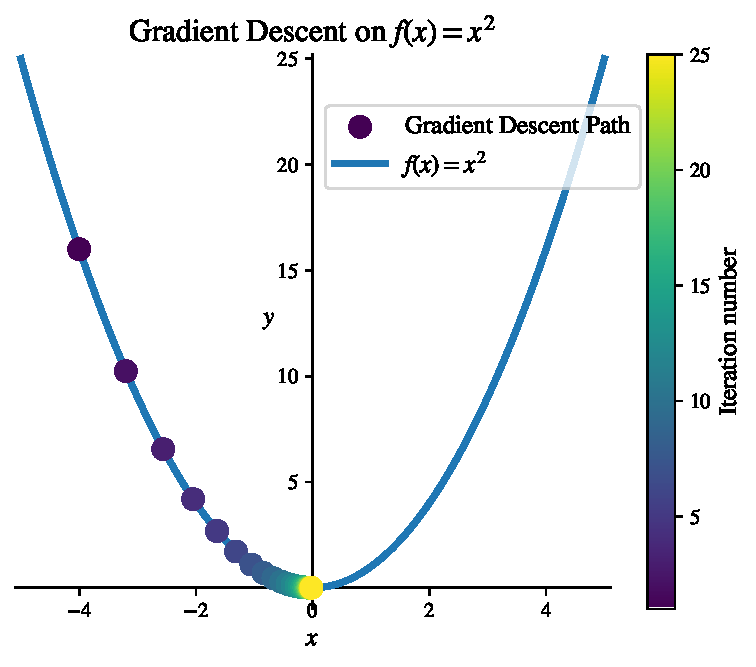
\includegraphics[width=0.68\textwidth]{figures/simple_gradient_descent_x^2.pdf}
    \caption{Gradient Descent on the function $f(x)=x^2$, starting from $x_0 = -4$ with $\eta = 0.01$, ran for 30 iterations.}
    \label{fig:simple_gradient_descent}
\end{figure}
For this simple example the iteration converged quickly, reaching a absolute value less than 0.001 after only 27 iterations. Gradient descent is not always this efficient. 

The two natural weaknesses of gradient descent are neatly explained in \parencite[p.~65--71]{MLRefined}. The first stems from the gradient always being perpendicular to the contour line. This is easily proved through parameterization.


\begin{lemma}
    Let $w(t)$ be a parametrization of a countour surface for a differentiable function $f: X^n \rightarrow Y$. Then $\nabla f \perp w(t) $ 
\end{lemma}

\begin{proof}
$$f(w(t)) = C \Rightarrow \frac{d}{dt} f(w(t)) = 0 \Rightarrow \nabla f(w(t)) \cdot \frac{\partial w(t)}{\partial t} = 0$$
The result follows from $\frac{\partial w(t)}{\partial t}$ being parallel to the contour
\end{proof}

This may lead to Zig-zagging behavior for ill conditioned problems.

\begin{figure}[H]
    \centering
    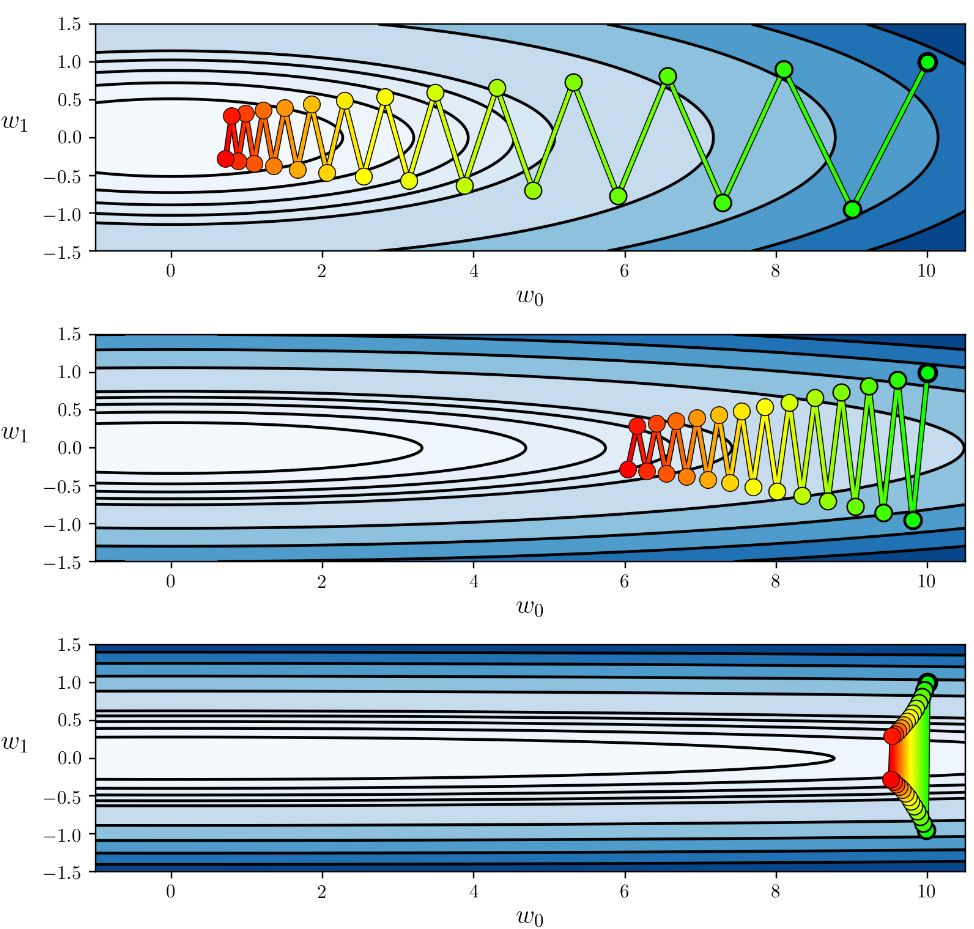
\includegraphics[width=0.9\textwidth]{Project2/figures/Gradient_descent_zigzag.jpeg}
    \caption{Figure 3.13 \parencite[p.~68]{MLRefined} illustrating the zig-zagging behavior
of gradient descent.}
    \label{fig:zigzagGradientDescent}
\end{figure}

The other challenge of gradient descent is its slow crawling behaviour in flatter regions of a function such as saddle points.  
This is nicely illustrated by 50 iterations with $\eta = 0.1$ on the function 
\[g(w) =  max^2(0, 1 + (3w - 2.3)^3) + max^2(0, 1 + (-3w + 0.7)^3)\]

\begin{figure}[H]
    \centering
    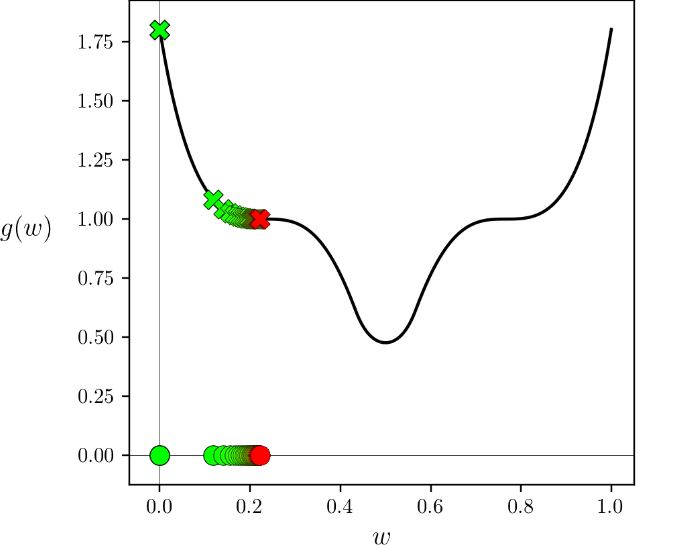
\includegraphics[width=0.7\textwidth]{Project2/figures/Gradient_descent_saddle_crawl.jpeg}
    \caption{Figure 3.14 \parencite[p.~70]{MLRefined} illustrating the slow crawling behaviour
of gradient descent.}
    \label{fig:CrawlGradientDescent}
\end{figure}

\begin{comment}
When performing gradient descent for machine learning the function we are minimizing is the cost function. A measure of the distance between predicted and observed outputs. It is important to note that this function is defined by 
\end{comment}

\subsubsection{Stochastic gradient descent}
Recall that the cost function is defined by the difference between our predictions and observed values. A large dataset thus gives a computationally expensive cost function and corresponding gradient. To combat this Stochastic gradient descent (or SGD) introduces the concept of batching.


Instead of computing the cost and corresponding gradient for all data points, we instead choose $M$ points at random without replacement (a batch), to calculate from. The cost surface achieved by this is truly a different surface from the one achieved by using all the data points, but the number of features and thus the dimentionality, is the same. For this method to work we are banking on there being enough overlap between the samples such that the gradient is expected to point in the same direction when calculated for all data points.


It is common practice to organize our algorithm in a double loop. If we have $n$ samples in total the inner loop iterates over $\lfloor\frac{M}{n} \rfloor$. That is the number of batches that fit in our dataset. And the outer loop iterates over the number of epochs. Which is an arbitrary number. In the special case of $M = n$, there is only one batch and SGD becomes "vanilla" gradient descent. 

\newpage

\begin{algorithm}[hbt!]
\caption{Stochastic Gradient Descent with Batching}\label{alg:SGD}
\KwData{Dataset D={$x_1,...,x_n$}, Learning rate $\eta$, Batch Size M, No. of Epochs E}
\KwResult{Model Parameters w}
\For{i in range(E)}{
    batches = create\_batches(D, M)\;
  \For{j in range(n//M)}{
    batch = batches[j]\;
    gradient = compute\_gradient(batch, w)\;
    w = w - $\eta$ $\cdot$ gradient\;
  } 
}
\end{algorithm}
 
Let $\mathbf{x_i}$ be the $i_{th}$ batch and $i=1,...,m$, then we can rewrite (\ref{eq:gradient_descent}) as
\begin{align*}
        \mathbf{w_{j+1}} = \mathbf{w_j} - \eta_j\nabla\mathbf{f_i(x_i)}
\end{align*}
where $j=1,...,m \cdot \#epochs$. Notice that the gradient is indexed as it is defined from the data points in the batch.

As stated above subsection, gradient descent finds the local minima $f(\xi)$ by exploration. This is beneficial for convex functions or if the local minima is already known to be the global minima. For non-convex functions or in the case where the global minima is not known (which is the case most of the time), SGD introduces more exploration. This means that instead of getting stuck in a local minima, by randomness, there is a higher probability of finding the global minima. SGD also have an added bonus that it is dependent on the batch size rather than the data set size. Thus the learning rate can still converge, even if the data set is large.

It is important to keep in mind that for the following descent methods we can define their corresponding stochastic counterparts in the same way as we did for gradient descent. And  that gradient descent and stochastic gradient descent is sometimes used to refer to the family of optimizers and their stochastic counterparts.

\subsubsection{Momentum based gradient descent}
Momentum is an added parameter meant to address these issues of vanilla gradient descent. The iteration is defined as

\begin{equation}
\begin{aligned} 
    \mathbf{w}_{k+1} &= \mathbf{w}_k + \mathbf{v}_{t+1}, \\
    \mathbf{v}_{t+1} &= \rho \mathbf{v}_t - \eta \mathbf{g}_k, \qquad \mathbf{v}_0 = 0 
\end{aligned}
\label{eq:momentum_eq}
\end{equation}


$\mathbf{v}$ is called the velocity term and $\rho$ is the momentum parameter. $\rho$ can be thought of as the velocities resistance to change while the learning rate ($\eta$) characterizes the influence of the gradient. An intuitive analogy is to think of our descent algorithm as a particle moving on the surface we wish to minimize. The gradient is the force acting on our particle ($\eta$ is its amplifier) and $\rho$ is the mass of the particle. This way our particle might be able to roll past the saddle point in \autoref{fig:CrawlGradientDescent} and obtain a less "zig-zaggy" path in \autoref{fig:ZigZagMomentumGradientDescent}.

Here we see momentum gradient descent performed on the same ill conditioned problem as the first panel of \autoref{fig:ZigZagMomentumGradientDescent} with $\rho$ equal to $0, 0.2, 0.7$ respectively

\begin{figure}[H]
    \centering
    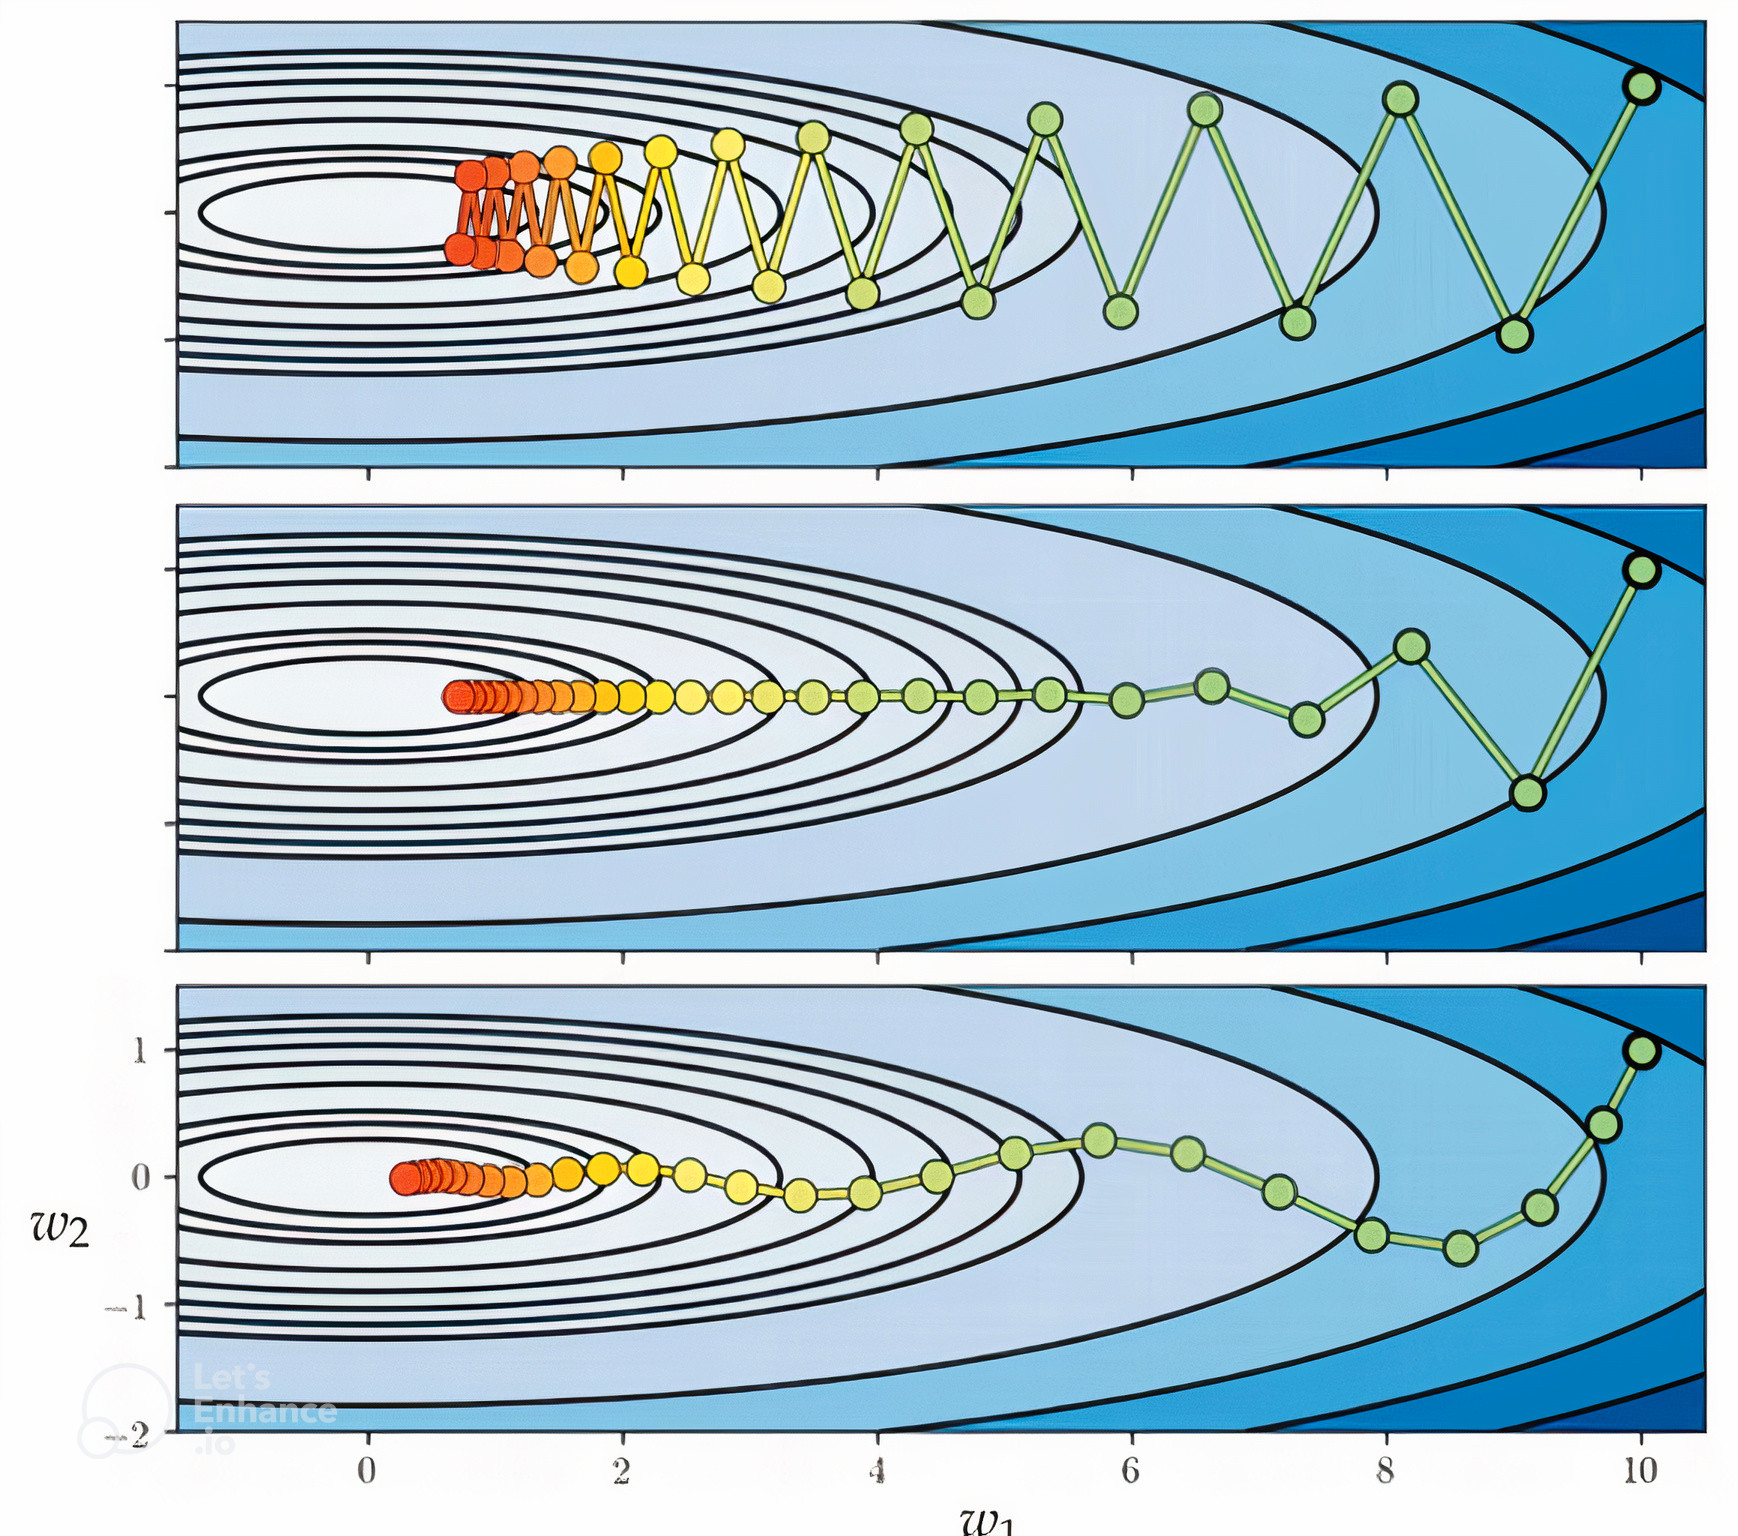
\includegraphics[width=0.8\textwidth]{Project2/figures/momentum_based_gradient_descent_less_zig.jpg.jpg}
    \caption{Figure A3 \parencite[p.~478]{MLRefined} The zig-zagging behavior of gradient
descent can be ameliorated using the momentum-accelerated gradient descent}
    \label{fig:ZigZagMomentumGradientDescent}
\end{figure}


\subsubsection{AdaGrad}
The Adaptive gradient optimizer, or AdaGrad was introduced by \textcite{duchi2011adaptive} and its update rule is given by

\[ w_{k+1}= w_{k}-\eta \hspace{1mm} diag\left(\mathbf{G_{k}}\right)^{-1/2} \odot \mathbf{ g_k} \]
where $\odot$ is the Hadamard product and $G_k$ is the sum of the outerproducts of the previous gradients
\begin{equation*}
    G_k = \sum_{i = 0}^k \mathbf{g_i} \mathbf{g_i^T}
\end{equation*}

 We thus have that $diag\left(G_{k}\right)^{(n)}$ ( the $n^{th}$component of $diag\left(G_k\right)$) is the sum of the squares of the previous gradients in direction $n$
 \[
 diag\left(G_{k}\right)^{(n)} = \sum_{i=0}^k  \left(g_k^{(n)}\right)^2 
 \]

 Normally a small numerical stabiliser is added to $G_k$ to avoid division by zero
 \[
 w_{k+1}^{(n)}= w_{k}^{(n)}- \frac{\eta}{ \sqrt{\delta+diag\left(G_{k}\right)^{(n)}}} \odot g_k^{(n)}
 \]
 

As $diag\left(G_k\right)^{(n)}$ increases, the step size in direction $n$ decreases, which reduces the emphasis on that particular direction as it is traversed. This is the core concept of AdaGrad's design. AdaGrad is most effective when two conditions are met: first, when we need to move the same distance in each dimension, and second, when we have an appropriate choice of $\eta$. Opting for a too small $\eta$ could result in the algorithm converging very slowly or coming to a halt due to the decaying step size. Conversely, selecting a too large $\eta$ could lead to also sluggish convergence. Thus, selecting an appropriate value of $\eta$ is vital to ensuring efficient functioning of the algorithm. 


\subsubsection{RMSprop}
RMSprop, root mean square propagation, was first introduced in 2012, in lecture 6 of the Coursera course ``Neural Networks for Machine Learning" by Geoff Hinton
\parencite{NNforML-Lecture6} It's update rule is defined as 

\begin{align*}
    \mathbf{v_{k+1}} =& \rho \mathbf{v_{k}} + (1-\rho) \mathbf{g_k}^{\circ 2}\\
    w_{k+1}^{(n)} =& w_k^{(n)} - \frac{\eta}{  \sqrt{\delta + v_{k+1}^{(n)}}} g_k^{(n)}
\end{align*}

 We have chosen to only give the element wise update rule, as for RMSprop, as the vector notation for the final equation is not very pretty. $\delta$ is a numerical stabilizer, $0\leq \beta \leq 1$ and $\mathbf{v_0}$ is usually initialised to the zero vector.
\par
\vspace{1mm}
Like AdaGrad the update keeps some sort of memory of previous gradients. Where $\beta$ can be thought of as the strength of the memory; how much of the previous iterations should impact the next. This allows for some of the same benefits as AdaGrads decaying learningrate.

\subsubsection{ADAM}
Adaprive moment estimation, most commonly known as ADAM. Is a optimization algorithm which combines the some of the aspects from RMSprop with momentum. It's update is given by
\begin{align*}
    \mathbf{m_{k+1}} =& \frac{\rho_1 \mathbf{m_k} + (1- \rho_1) \mathbf{g_k}}{\left(1 - \rho_1^{k+1}\right)}\\
    \mathbf{v_{k+1}} =& \frac{\rho_2 \mathbf{v_k} + (1-\rho_2) \mathbf{g_k}^{\circ 2}}{\left(1-\rho_2^{k+1}\right)}\\
    w_{k+1}^{(n)} =& w_k^{(n)} - \frac{\eta}{ \sqrt{\delta+v_{k+1}^{(n)}}} m_{k+1}^{n}
\end{align*}

Here $0 \leq \beta_1,\beta_2 < 1$ 
\par
\vspace{1mm}
Notice that the denominator of $\mathbf{m_{k+1}}$ and $\mathbf{v_{k+1}}$ starts somewhere in $(0,1]$ and then increases to 1 as $k \to \infty$. This gives an amplification of $\mathbf{m_k}$ and $\mathbf{v_k}$, which subsides for larger $k$. This is meant to alleviate a bias towards zero as  $\mathbf{m_0}, \mathbf{v_0} = 0$ \parencite[Section 3]{kingma2014adam}

%It may be tempting to conclude that every subsequent algorithm is superior to its predecessor. However, this is not strictly true.
\vspace{2mm}
Optimization algorithms can be used to minimize any specific function. However, the latter three are all designed for minimizing a particular set of functions; the cost functions of Artificial Neural Networks (ANNs). These cost functions measure the error made by ANNs in predicting observed values from input data. How these predictions are made and adjusted is the topic of section 2.4






\subsection{Neural Networks}
% Neural networks are computational systems inspired by the networks of neurons in the brain.

% A neural network mainly consists of an input layer of nodes, a set of weights, an activation function, a hidden layer of nodes and a layer of output nodes. The input nodes are usually called features. Each node is connected to all nodes in the next layer and the edge between them have a weight on it. In the next layer, each input to the node is multiplied with its own weight and then summed together. These nodes are usually what we would call an artificial neuron.\\
% Let $f: X \rightarrow X$ be a function (?), then we can define the artificial neuron as
% \begin{equation*}
%     y = f\left( \sum_{i=1}^{n}w_ix_i \right)
% \end{equation*}
% \\
% $\ldots$\\
Neural networks are computational systems inspired by the networks of neurons within the brain. In the brain, when a neuron receives an electrical impulse above a certain threshold, it sends an electrical signal to the neurons connected to it, causing a chain reaction. In order to mimic this, an artificial neural network is set up with a number of layers, each with a set of artificial neurons. The first layer is commonly called the input layer, which is followed by a number of hidden layers, culminating in the final layer called the output layer.

\begin{figure}[ht]
\centering
\def\layersep{2.5cm}
\def\nodeinlayersep{1.2cm}
\begin{tikzpicture}[shorten >=1pt,->,draw=black!50, node distance=\layersep]
    \tikzstyle{every pin edge}=[<-,shorten <=1pt]
    \tikzstyle{neuron}=[circle, fill=black!25,minimum size=20pt,inner sep=0pt]
    \tikzstyle{input neuron}=[neuron, fill=red!50];
    \tikzstyle{output neuron}=[neuron, fill=orange!50];
    \tikzstyle{hidden neuron}=[neuron, fill=blue!50, minimum size=20pt];
    \tikzstyle{hidden neuron2}=[neuron, fill=blue!50, minimum size=20pt];

    \foreach \name / \y in {0,...,2}
        \node[input neuron] (I-\name) at (0,-\y) {};

    \foreach \name / \y in {0,...,3}
        \path[yshift=0.5cm]
            node[hidden neuron] (H1-\name) at (\layersep,-\y cm) {};

    \foreach \name / \y in {0,...,3}
        \path[yshift=0.5cm]
            node[hidden neuron2] (H2-\name) at (2*\layersep,-\y cm) {};    

    \foreach \name / \y in {0,...,1}
        % \node[output neuron,pin={[pun edge={->}]right:Output \#\y}, right of=H2-2] (O-\name) at (3*\layersep, -\y cm) {};
        \path[yshift=-0.5cm]
            node[output neuron] (O-\name) at (3*\layersep, -\y cm) {};


    \foreach \source in {0,...,2}
        \foreach \dest in {0,...,3}
            \path (I-\source) edge (H1-\dest);

    \foreach \source in {0,...,3}
        \foreach \dest in {0,...,3}
            \path (H1-\source) edge (H2-\dest);

    \foreach \source in {0,...,3}
        \foreach \dest in {0,...,1}
            \path (H2-\source) edge (O-\dest);
\end{tikzpicture}
\caption{Illustration of a fully connected feed-forward neural network with an input layer (red), two hidden layers (blue) and an output layer (orange).}
\label{fig:SimpleFFNN}
\end{figure}

The \textit{feed-forward} neural network (FFNN), was the first, and perhaps simplest, artificial neural network (\textbf{SOURCE}). Each node is connected to nodes in the next layer, with a weight $w \in \mathbb{R}$ attached to each edge, representing the strength of the connection between them. Additionally, we attach a bias $b \in \mathbb{R}$ to the node itself, also refereed to as the offset. Henceforth, we describe the \textit{fully connected} feed-forward neural network, where the nodes are connected to \textit{all} nodes in the next layer, illustrated in \autoref{fig:SimpleFFNN}.


Information in this network moves from left to right. The value of a node is dependent on the weights and values of the previous layer, as well as the bias. Let $N_l \in \mathbb{N}$ be the number of nodes in layer $l$ with the input layer being $l = 0$. We then calculate
\begin{equation*}
    z_{i}^1 = \sum_{j = 0}^{N_0 - 1} w_{ij}^1 x_j + b_i^1 \qquad \textnormal{for} \ i = 0, 1, \ldots, N_1 - 1,
\end{equation*}
with $w^l_{ij}$ being the weight connecting node $i$ in layer $l$ and node $j$ in layer $l-1$, $b_i^l$ the bias of node $i$ and $x_j$ the $j^{th}$ input. We call $z$ the activation value. Let $f^l: \mathbb{R} \to \mathbb{R}$ be a function, called the activation function for the $l^{\text{th}}$ layer. We calculate the output of the node by $a_i^l = f^l(z_i^l)$. For the following layers, we calculate a \textit{feed-forward pass}
\begin{equation*}
    a_i^l = f^l(z_{i}^l) = f^l \left( \sum_{j = 0}^{N_l - 1} w_{ij}^l a_j^{l-1} + b_i^{l} \right) \qquad \textnormal{for} \ i = 0, 1, \ldots, N_l - 1,
\end{equation*}
illustrated in \autoref{fig:FeedForward}.

\begin{figure}[ht]
\centering
\def\layersep{3cm}
\def\nodeinlayersep{2cm}
\begin{tikzpicture}[shorten >=1pt,->,draw=black!50, node distance=\layersep]
    \tikzstyle{every pin edge}=[<-,shorten <=1pt]
    \tikzstyle{neuron}=[circle, fill=black!25,minimum size=25pt,inner sep=0pt]
    \tikzstyle{input neuron}=[neuron, fill=red!50];
    \tikzstyle{output neuron}=[neuron, fill=orange!50];
    \tikzstyle{hidden neuron}=[neuron, fill=blue!50];

    % Input nodes
    \foreach \name / \y in {0,...,1}
        \node[input neuron] (I-\name) at (0,-\y * \nodeinlayersep) {$x_\y$};

    % Hidden layer
    \foreach \name / \y in {0,...,1}
        \node[hidden neuron] (H-\name) at (\layersep,-\y * \nodeinlayersep) {$a_\y^1$};

    % Output node
    \path[yshift=-0.5 * \nodeinlayersep]
        node[output neuron] (O-0) at (2*\layersep, 0 cm) {$a_0^2$};

    \path[->] 
        % Weights from first input
        (I-0) edge [->] node [midway, above] {$w^1_{0, 0}$} (H-0)
        (I-0) edge [->] node [midway, above] {$w^1_{0, 1}$} (H-1)
        % Weights from second input
        (I-1) edge [->] node [midway, below] {$w^1_{1, 0}$} (H-0)
        (I-1) edge [->] node [midway, below] {$w^1_{1, 1}$} (H-1)
        % Weights to output
        (H-0) edge [->] node [midway, above] {$w^2_{0, 0}$} (O-0)
        (H-1) edge [->] node [midway, below] {$w^2_{1, 0}$} (O-0);

    
    \foreach \source in {0,...,1}
        \foreach \dest in {0}
            \path (H-\source) edge (O-\dest);

    \path[->]
        (H-0) edge [loop above] node [above] {$f\left(z_0^1\right)$} ()
        (H-1) edge [loop below] node [below] {$f\left(z_1^1\right)$} ()
        (O-0) edge [loop above] node [above] {$f\left(z_0^2\right)$} ();

    \node (BH-0) at (0.5*\layersep,  0.5*\nodeinlayersep) {$b_0^1$};
    \node (BH-1) at (0.5*\layersep, -1.5*\nodeinlayersep) {$b_1^1$};
    \node (BO-0) at (1.5*\layersep, -0.5*\nodeinlayersep) {$b_0^2$};

    \path[->]
        (BH-0) edge (H-0)
        (BH-1) edge (H-1)
        (BO-0) edge (O-0);
\end{tikzpicture}
\caption{Illustration of a feed-forward pass in a neural network with two inputs (red), two hidden nodes (blue), and one output node (orange).}
\label{fig:FeedForward}
\end{figure}

We gather the weights connecting the $l^{th}$ and $(l-1)^{th}$ layers in a $N_{l} \times N_{l-1}$ matrix $\mathbf{W}_l$, and the biases and outputs in $N_l \times 1$ column vectors $\mathbf{b}_l, \mathbf{y}_l$ as follows.
\begin{equation*}
    \mathbf{W}_l = 
    \begin{bmatrix}
        w_{0,0} & w_{0,1} & \ldots & w_{0,N_{l-1}} \\
        w_{1,0} & w_{1,1} & \ldots & w_{1,N_{l-1}} \\
        \vdots & \vdots & \ddots & \vdots \\
        w_{N_{l},0} & w_{N_{l},1} & \ldots & w_{N_{l},N_{l-1}} \\
    \end{bmatrix}
    \qquad
    \mathbf{b}_l =
    \begin{bmatrix}
        b_0^l \\ b_1^l \\ \vdots \\ b_{N_l}^l
    \end{bmatrix}
    \qquad
    \mathbf{y}_l =
    \begin{bmatrix}
        y_0^l \\ y_1^l \\ \vdots \\ y_{N_l}^l
    \end{bmatrix}
\end{equation*}
We can then simplify the summation to get $\mathbf{z}_l = \mathbf{W}_l \mathbf{y}_{l-1} + \mathbf{b}_l$. We then extend the function $f^l: \mathbb{R} \to \mathbb{R}$ to the function $F^l: \mathbb{R}^{N_l \times 1} \to \mathbb{R}^{N_l \times 1}$ by defining
\begin{equation*}
    F^l(\boldsymbol{x}) = \left[ f^l \left( x_0 \right), \ f^l \left( x_1 \right), \ \ldots, \ f^l \left( x_{N_l - 1} \right) \right]^T,
\end{equation*}
such that the function operates elementwise. For simplicity sake, this function $F^l$ will also be notated $f^l$.

We define the realization of our neural network as the function $\mathcal{N}: \mathbb{R}^{N_0 \times 1} \to \mathbb{R}^{N_h \times 1}$, with $h$ being the output layer as
\begin{equation*}
    \mathcal{N}(\boldsymbol{x}) =
    f^h\left(
    \mathbf{W}_h f^{h-1} \left(
    \mathbf{W}_{h-1}f^{h-2} \left(\ldots f^1\left( \mathbf{W}_1 \boldsymbol{x} + \mathbf{b}_1 \right) \right)
    + \mathbf{b}_{h-1} \right) 
    + \mathbf{b}_h \right).
\end{equation*}
Defining the function $\mathcal{A}^l: \mathbb{R}^{N_{l-1} \times 1} \to \mathbb{R}^{N_{l}}$ as the function
\begin{equation*}
    \mathcal{A}^l (\boldsymbol{x}) = \mathbf{W}_l \boldsymbol{x} + \mathbf{b}_l,
\end{equation*}
we can simplify our notation by noting that $\mathcal{N}$ is a composition of functions
\begin{align*}
    \mathcal{N} &= f^h \circ \mathcal{A}^h \circ f^{h-1} \circ \mathcal{A}^{h-1} \circ \ldots \circ f^1 \circ \mathcal{A}^1 \\
    &= \bigcirc_{i = 1}^h f^{i} \circ \mathcal{A}^{i}.
\end{align*}

The Universal Approximation Theorem states that a neural network with even a single hidden layer, can approximate a continuous function on a compact subset arbitrarily well with an arbitrary number of hidden nodes given a fitting choice for the activation function \parencite{universalapprox}. The proof of this theorem falls outside the scope of this project, but we highly recommend i.e. \textcite{Guliyev2015ASH} or \textcite{universalapprox} if you have a passing interest in analysis. As we will see, our choice of activation function matters greatly.

\subsubsection{Activation functions}
For the sake of brevity, we restrict our self to one activation function for the hidden layers, and one for the output layer. To motivate our choice of activation function, we begin with the definition of a linear operator from real analysis \parencite[p.~150]{lindstrom2017spaces}.

\begin{definition}
    Assume that $V$ and $W$ are two vector spaces over $\mathbb{R}$. A function $A: V \to W$ is called a \textit{linear operator} (or a \textit{linear map}) if it satisfies:
    \begin{enumerate}[label=(\roman*)]
        \item $A(\alpha\boldsymbol{u}) = \alpha A(\boldsymbol{u}$) for all $\alpha \in \mathbb{R}$ and $\boldsymbol{u} \in V$.

        \item $A(\boldsymbol{u} + \boldsymbol{v}) = A(\boldsymbol{u}) + A(\boldsymbol{v})$ for all $\boldsymbol{u}, \boldsymbol{v} \in V$.
    \end{enumerate}
\end{definition}

\begin{theorem}[Composition of linear operators]
    Assume that $U, V, W$ are vector spaces over $\mathbb{R}$ and that $A: U \to V$, $B: V \to W$ are linear operators. Then $B \circ A$ is a linear operator.
    \label{thm:Linear}
\end{theorem}
\begin{proof}
    Let $\boldsymbol{u}, \boldsymbol{v} \in V$, $\alpha, \beta \in \mathbb{R}$. Then
    \begin{align*}
        B(A(\alpha \boldsymbol{u} + \beta \boldsymbol{v})) &= B(\alpha A(\boldsymbol{u}) + \beta A(\boldsymbol{v}))
        = \alpha B(A(\boldsymbol{u})) + \beta B(A(\boldsymbol{v})),
    \end{align*}
    showing that $B \circ A$ is indeed a linear operator.
\end{proof}

Due to \autoref{thm:Linear}, if we were to choose a linear activation function for the hidden layer, $\mathcal{N}$ would just be a composition of linear operators, and therefore be linear itself. We would then not get any benefit from adding multiple hidden layers, as it could just be represented as one linear operation. This greatly restricts the hypothesis space, which is why we opt for non-linear activation functions \parencite[p.~72]{CholletFrancois2018DlwP}.
% \parencite[p.~72]{CholletFranccois2018DlwP}

A common choice, and the one first presented in \textcite{universalapprox}, is a so called sigmoidal function $\sigma$. A sigmoidal function is a function $\sigma: \mathbb{R} \to \mathbb{R}$ which satisfies
\begin{equation*}
    \lim_{t \to +\infty} \sigma(t) = 1 \qquad \textnormal{and} \qquad \lim_{t \to -\infty} \sigma(t) = 0.
\end{equation*}
A simple function which satisfies this, is the $(0,1)$-clip function, defined by
\begin{equation*}
    f(x) = 
    \begin{cases}
        1 & \textnormal{for } x \geq 1 \\
        x & \textnormal{for } x \in (0,1) \\
        0 & \textnormal{for } x \leq 0
    \end{cases}.
\end{equation*}
The most common choice however is perhaps the standard logistic function \parencite{jentzen2023mathematical}, often just called the sigmoid function, defined by
\begin{equation*}
    f(x) = \frac{1}{1 + e^{-x}}.
\end{equation*}
Both of these functions are clearly sigmoidal, illustrated in the plot in \autoref{fig:sigmoid}.

\begin{figure}[ht]
    \centering
    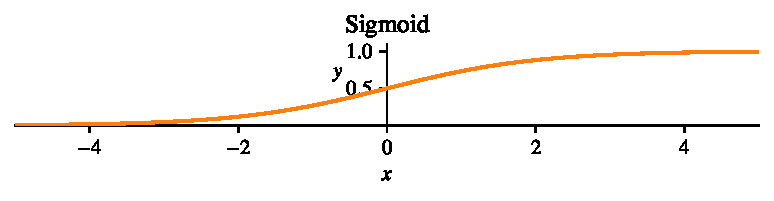
\includegraphics[width=.7\textwidth]{activators/sigmoid.pdf}
    \caption{A plot of the sigmoid and $(0,1)$-clip activation functions on $[-4, 4]$.}
    \label{fig:sigmoid}
\end{figure}

% However, the activation functions do not have to be sigmoidal in order to satisfy the requirements for the Universal Approximation Theorem. In fact, it is enough to require that the activation function is non-polynomial \parencite{nonpolynomial}. (\small{venter på svar fra Morten, virker for godt til å være sant}) 

Another commonly used activation function is the rectified linear unit (ReLU), defined by
\begin{equation*}
    f(x) = \max(0, x) = \frac{x + |x|}{2} =
    \begin{cases}
        x & \textnormal{if } x \geq 0 \\
        0 & \textnormal{if } x < 0
    \end{cases}.
\end{equation*}
However, this function suffers from what some call dying ReLUs, where nodes in effect die by outputting constant $0$. To combat this, we introduce the leaky rectified linear unit (LReLU), defined by
\begin{equation*}
    f(x) =
    \begin{cases}
        x & \textnormal{if } x \geq 0 \\
        \gamma x & \textnormal{if } x < 0
    \end{cases}.
\end{equation*}
for some positive $\gamma \in \mathbb{R}$. 

\begin{figure}[ht]
    \centering
    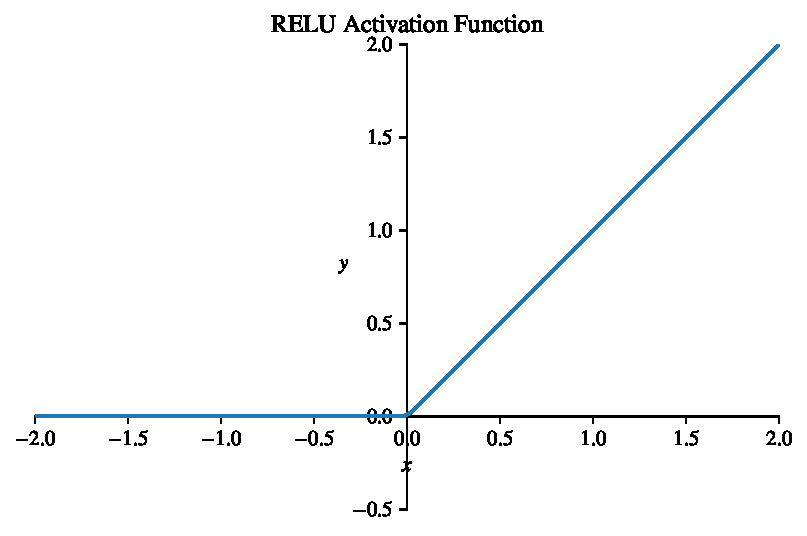
\includegraphics[width=.7\textwidth]{activators/RELU.pdf}
    \caption{A plot of rectified linear unit (ReLU) activation function on $[-2, 2]$.}
    \label{fig:RELU}
\end{figure}

\begin{figure}[ht]
    \centering
    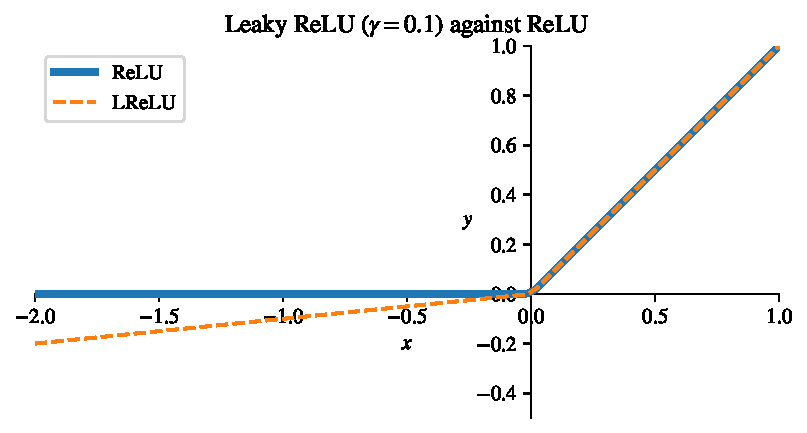
\includegraphics[width=.7\textwidth]{activators/LReLU.pdf}
    \caption{A plot of leaky rectified linear unit (LRELU) activation function on $[-2, 1]$, with $\gamma=0.1$, against RELU.}
    \label{fig:LRELU}
\end{figure}


Two other important functions that are particularly used on the output layer for multi-class classification problems, are the $\argmax$ and $softmax$ functions.

The $\argmax$ function delivers the index or position associated with the highest value from a numeric input vector. If  each node in the output layer denotes the models predicted probability of an input being classified in the corresponding class, it becomes clear that the $\argmax$ function essentially provides the predicted class or classification. This function is however, is not differentiable and therefore is not suited for training. Which will be clear by section 2.3.2.

The $softmax$ function is used to convert any vector to a valid discrete probability distribution. It is given by
\[
softmax(\textbf{z}) = \begin{bmatrix}
\frac{e^{z_1}}{\sum_i e^{z_i}} \\
\vdots \\
\frac{e^{z_n}}{\sum_i e^{z_i}}
\end{bmatrix} = \textbf{a}
\]
It keeps the sorted order of the input vector. That is if $z_i < z_j$ then $a_i < a_j$. It also satisfies
\[
\sum_{i=1}^n a_i = 1
\]



\subsubsection{Minimizing the cost function: Backpropagation}

Backpropagation serves as the heart of model optimization. As the name implies, it involves a backwards pass through our Artificial Neural Network (ANN). To understand its operation, we need to consider a model, referred to here as $\mathcal{N}$. After computing the output for a given input variable, $\boldsymbol{x}$, denoted by $\mathcal{N}(\boldsymbol{x})$, it becomes inherently natural to assess the performance of our model. Specifically, we want to compute the loss emerging from deviations between the model's output and the expected values

\[
L(\mathcal{N}(\boldsymbol{x}), \mathbf{y})
\]
The mean over $n$ such losses gives us the cost function
\[
C(\mathcal{N}, \boldsymbol{x}^*, \mathbf{y}^*) = \frac{1}{n} \sum_{i=0}^{n}L(\mathcal{N}(\boldsymbol{x}^{(i)}), \mathbf{y}^{(i)})
\]
Here we let $\mathbf{x}^*$ and $\mathbf{y}^*$ denote the matrices containing the column vectors $\mathbf{x}^{(i)}$ and $\mathbf{y}^{(i)}$. These matrices are commonly referred to as our labeled data or our training data. This cost function is our optimization problem, the function we wish to minimize. 

\[
\argmin_{\mathcal{N}} C(\mathcal{N}, \boldsymbol{x}^*, \mathbf{y}^*) 
\]
$\mathcal{N}$ consists of three components: our weights, biases and activation functions. Minimizing with respect to the activation functions is not necessary, as by the Universal Approximation Theorem, there are many that will suffice. By minimizing with respect to the weights and biases we get the back propagation algorithm.

Letting $\eta$ and $\mu$ encompass all the different learning rates by our methods in section 2.2 we get the general iteration on layer $l$
\begin{align*}
    \hat{w_{i,j}^{l}} =\hspace{1mm}&
    w_{i,j}^{l} - \eta \frac{\partial C}{\partial {w_{i,j}^{l}}}\\
    \hat{b_i^{l}} =\hspace{1mm}& b_i^{l} - \mu  \frac{\partial C}{\partial b_i^l} 
\end{align*}

Here we are taking some notational liberty in the use of partial derivatives. As we'll see these are functions of the weights, the pre-activated and the activated values of the network, and are of course evaluated at the current values for a iteration. 

 We return to $a_i^l$ begin the value of node $i$ in layer $l$ and $z_i^l$ the value before activation. Then for some arbitrary layer $l$ we get, by the chain rule

\begin{align}
    \frac{\partial C}{\partial w_{i,j}^l} =& \frac{\partial C}{\partial a_i^l} \frac{\partial f^l}{\partial z_i^l} \frac{\partial z_i^l}{\partial w_{i,j}^l} \label{eq:1} 
    \\
    \frac{\partial C}{\partial b_i^l} = & \frac{\partial C}{\partial a_i^l} \frac{\partial f^l}{\partial z_i^l} \frac{\partial z_i^l}{\partial b_i^l} \label{eq:2} 
\end{align}
The third factors of these products simplifies to

\begin{align}
    \frac{\partial z_{i}^l }{\partial w_{i,j}^l} = &  \frac{\partial}{\partial w_{i,j}^l} \sum_{k = 0}^{N_l - 1} w_{i,k}^L a_k^{l-1} + b_i^l = a_j^{l-1} \label{eq:3} \\
    \frac{\partial z_i^l}{\partial b_i^l} = &  1 \label{eq:4} 
\end{align}

\noindent
The second, $\frac{\partial f^l}{\partial z_i^l}$ can simplified to $f^{l'}(z_i^l)$ whenever the activation function $f^l$ is a function of just one variable. 


\begin{figure}[ht]
\centering
\def\layersep{2.5cm}
\def\nodeinlayersep{1.2cm}
\begin{tikzpicture}[shorten >=1pt,->,draw=black!50, node distance=\layersep]
    \tikzstyle{every pin edge}=[<-,shorten <=1pt]
    \tikzstyle{neuron}=[circle, fill=black!25,minimum size=20pt,inner sep=0pt]
    \tikzstyle{hidden neuron}=[neuron, fill=blue!50, minimum size=20pt];
    \tikzstyle{hidden neuron2}=[neuron, fill=blue!50, minimum size=20pt];
    \tikzstyle{hidden neuron opaque}=[neuron, fill=blue, minimum size=20pt, opacity=0.2];  % New style for opaque neurons


    \foreach \name / \y in {1}
        \path[yshift=0.5cm]
            node[hidden neuron] (H1-\name) at (\layersep,-\y cm) {$a^l_i$};

    \foreach \name / \y in {0,2,3} 
        \path[yshift=0.5cm]
            node[hidden neuron opaque] (H1-\name) at (\layersep,-\y cm) {};

    \foreach \name / \y in {0,...,3}
        \path[yshift=0.5cm]
            node[hidden neuron2] (H2-\name) at (2*\layersep,-\y cm) {};    

    % Labels for the layers
    \node[above of=H1-0, node distance=11mm] (label1) {$l$};
    \node[above of=H2-0, node distance=11mm] (label2) {$l+1$};

     \node[above of=H1-0, node distance=7mm] (label1) {$\vdots$};
    \node[above of=H2-0, node distance=7mm] (label2) {$\vdots$};
    \node[below of=H1-3, node distance=7mm] (label1) {$\vdots$};
    \node[below of=H2-3, node distance=7mm] (label2) {$\vdots$};

    \foreach \source in {1}
        \foreach \dest in {0,...,3}
            \path (H1-\source) edge (H2-\dest);

\end{tikzpicture}
\caption{Illustration of Connections from one Neuron in a Neural Network}
\label{fig:Connections}
\end{figure}

\noindent
To see how $\frac{\partial C}{\partial a_i^l}$ expands. Consider \autoref{fig:Connections}. A change in $a_i^l$ will trickle down to the next layer. For a single edge we get
\[
\frac{\partial C}{\partial a_i^{l+1}} \frac{\partial a_j^{l+1}}{\partial a_i^l} =  \frac{\partial C}{\partial a_i^{l+1}} \frac{\partial f^{l+1}}{\partial z_j^{l+1}} w_{i,j}^{l+1}
\]

Summation over all the edges gives us $\frac{\partial C}{\partial a_i^l}$


\begin{align}
    \frac{\partial C}{\partial a_i^l} =  \sum_{i=0}^{N_{l+1}-1} \frac{\partial C}{\partial a_i^{l+1}} \frac{\partial f^{l+1}}{\partial z_j^{l+1}} w_{i,j}^{l+1} \label{eq:5} 
\end{align}


If $l$ is the final layer in the network $\frac{\partial C}{\partial a_i^l}$ is the partial derivative with respect to the multivariate function $C$ - no more chain rule with respect to other nodes.

Combining equation \eqref{eq:1} with \eqref{eq:3} and \eqref{eq:2} with \eqref{eq:4}. We get

\begin{align}
     \frac{\partial C}{\partial w_{i,j}^l} =& \frac{\partial C}{\partial a_i^l} \frac{\partial f^l}{\partial z_i^l} a_j^{l-1}\label{eq:6} 
    \\
    \frac{\partial C}{\partial b_i^l} = & \frac{\partial C}{\partial a_i^l} \frac{\partial f^l}{\partial z_i^l} \label{eq:7} 
\end{align}
Equations \eqref{eq:5} through \eqref{eq:7} form the backbone of the backpropagation algorithm. As we observe, equation \eqref{eq:5}, which is integral to both \eqref{eq:6} and \eqref{eq:7}, relies on the partial derivatives of the proceeding layer. After computing the forward pass and storing all the relevant network values, we can initiate the backpropagation process, moving from right to left, one layer at the time. This systematic approach allows us to calculate all the gradients necessary for our optimization algorithms.
\subsubsection{Automatic Differentiation}
Automatic Differentiation (AD), also known as algorithmic differentiation or computational differentiation, refers to a set of techniques to numerically evaluate partial derivatives. It differs from symbolic differentiation and numerical differentiation.

At a high level, automatic differentiation leverages the principle that any computational calculation, regardless of its complexity, carries out a series of basic arithmetic tasks (like addition, subtraction, multiplication, and division) and fundamental functions (such as exp, log, sin, cos, etc.). By repeatedly applying the chain rule to these processes, it is possible to compute partial derivatives \parencite{walther2007automatic} . These computations are not only precise to the working standard but also efficient. They require added storage requirements, in the worst case growing proportionally with number of operations in the function.
\parencite{baydin2018automatic}

The use of automatic differentiation techniques is most relevant for the calculation of $\frac{\partial C}{\partial a_i^L}$ for the final layer. As a single pass of reverse accumulation  allows us to calculate the partial derivatives with respect to the entire layer $a^L$. It is akin to what we do in back propagation. 



\subsubsection{Derivative of Binary Cross Entropy with respect to weights}
Recall the Loss and BCE cost function given by

\[
L(y, p) = -ylog(p) - (1-y)log(1-p)
\]

\[
C(\mathbf{y}, \mathbf{p}) = \frac{1}{n} \sum_{i=1}^{n} L(y_i, p_i)
\]


Let's look at the loss function first.
\[
\frac{\partial L(y,p)}{\partial p} = \frac{-y}{p} + \frac{1-y}{1-p} 
\]
For binary classification it's common to use the sigmoid as our activation function for the final layer to obtain a valid probability. Giving $\sigma(z) = p$ as the derivative is given by
\[
\sigma'(x) = \sigma(x)(1-\sigma(x))
\]
We get 

\begin{align*}
\frac{\partial L(y,p)}{\partial z} =& \frac{\partial L(y,p)}{\partial p} \frac{\partial p}{\partial z} \\
=& \left(\frac{-y}{p} + \frac{1-y}{1-p}\right) \left(p(1-p)\right)\\
=& -y(1-p) + (1-y)p\\
=& \hspace{1mm} p-y 
\end{align*}

Thus for the cost function with respect to the final layer of weights we get


\begin{align*}
    \frac{C}{\partial \mathbf{w^L}}  =& \hspace{1mm} \frac{\partial C}{\partial \mathbf{p}} \frac{\partial \mathbf{p}}{\partial \mathbf{w^L}} \odot \mathbf{w^L}
    \\
    =& \hspace{1mm} \frac{1}{n} \left( \mathbf{p} - \mathbf{y}\right) \odot \mathbf{w^L}
\end{align*}

This analytical expression is very convenient for backpropagation.


\newpage
\section{Method}
In order to verify that our methods work, we began with testing our gradient descent code with the polynomial
\begin{equation}\label{eq:simplepoly}
    f(x) = 4 - 3x + 2x^2.
\end{equation}
With this, we can more easily visualize and understand the difference between the various methods. We generated our data with 100 values for $\boldsymbol{x}_i \in N(0, 1)$, and added noise $\boldsymbol{\varepsilon}_i \in N(0, 1)$ to our values such that $\boldsymbol{y} = f(\boldsymbol{x}) + \boldsymbol{\varepsilon}$ seen in \autoref{fig:input_values}. Utilizing polynomial regression, our design matrix was then
\begin{equation}
    X = \begin{bmatrix}
        1 & x_0 & x_0^2 \\
        1 & x_1 & x_1^2 \\
        & \vdots & \\
        1 & x_{100} & x_{100}^2
    \end{bmatrix},
    \label{eq:design}
\end{equation}
seeking to find $\boldsymbol{\theta} = [\theta_0, \theta_1, \theta_2]^T$ minimizing our cost function. We utilized both OLS and Ridge regression, applying both the analytical derivative and automatic differentiation.

\begin{figure}[ht]
    \centering
    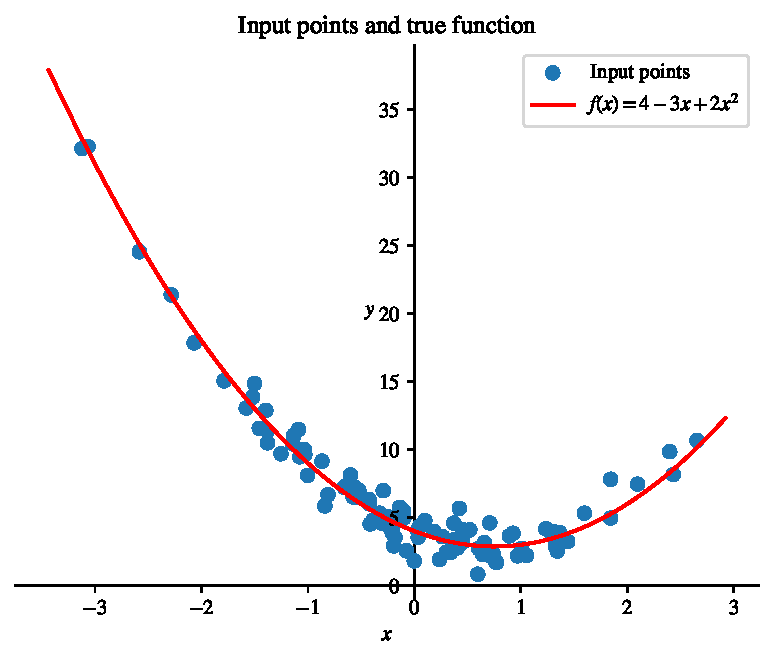
\includegraphics[width=0.7\textwidth]{Project2/figures/polynomial_grad/input_points.pdf}
    \caption{Values used for verifying gradient descent on $f(x) = 4 - 3x + 2x^2$.}
    \label{fig:input_values}
\end{figure}

With a better understanding of how gradient descent with the various methods works, we moved on to regression with a neural network. Here, we utilized Franke's function, defined by
\begin{equation*}
    \begin{split}
        f(x,y) & = \frac{3}{4}\exp\left(-\frac{(9x-2)^2}{4} - \frac{(9y-2)^2}{4}\right) + \frac{3}{4}\exp\left(-\frac{(9x+1)^2}{49} - \frac{(9y+1)}{10}\right) \\
        & + \frac{1}{2}\exp\left(-\frac{(9x-7)^2}{4} - \frac{(9y-3)^2}{4}\right) - \frac{1}{5}\exp\left(-(9x-4)^2 - (9y-7)^2\right).
    \end{split}
\end{equation*}
for $x,y \in [0,1]$. A major advantage with regression through the neural network is that we do not have to transform our inputs to a polynomial as in (\ref{eq:design}), instead allowing the network to learn the behaviour through the hidden layers. This has the advantage of not coaxing the network into fitting a polynomial. We therefore have only two input nodes for $x$ and $y$, with one output node outputting the predicted height $z$. We used 100 evenly spaced points in $[0,1]$ for our values of $x$ and $y$, transforming our inputs to a mesh grid giving $100 \times 100$ points.

For classification, we used the original Wisconsin Breast Cancer Dataset \parencite{breastcancerwisonsin}, attempting to predict from measurements of tumours whether they are malignant or benign. The dataset consists of 9 features, being labeled either 2 for benign or 4 for malignant. There are 699 data points, however 16 of them are missing some data and are thus excluded from our analysis.

\subsection{The code}
Our original implementation primarily used \verb|NumPy| for the linear algebra and \verb|autograd| for automatic differentiation. Due to computational concerns, it was then rewritten to primarily rely on \verb|JAX| \parencite{jax2018github}, which is a Google developed library combining \verb|XLA| and \verb|autograd| designed for high-performance computing. This has the advantage of being a lot faster, however leads to more verbose code. As an example, consider the sigmoid function implemented in \verb|JAX| and \verb|NumPy|.

\begin{minted}{python}
from jax import lax, jit
import numpy as np

@jit
def sigmoid_jax(X):
    return lax.reciprocal(lax.add(1.0, lax.exp(-X)))

def sigmoid_numpy(X): # NumPy equivalent
    return 1 / (1 + np.exp(-X))
\end{minted}

Note that we apply the \verb|@jit| operator to enable just-in-time compilation, which is a leading factor in the speedup. The sigmoid function is also a built-in function in \verb|JAX| under the name \verb|lax.logistic|, however we chose to use our own implementation to keep everything in the same style.

As \verb|jit| works poorly with classes, requiring methods to be completely functional in order to assure correct functionality, we chose to extract the most costly computations into their own functions, using pure python primarily for higher level bookkeeping. One of the trickier parts of porting to \verb|JAX| was that it has no built in method for elementwise differentiation. Thus to differentiate the hidden functions, which are performed elementwise, we used the following code.

\begin{minted}{python}
from jax import grad, vmap
from autograd import elementwise_grad

def derivate_jax(func):
    return vmap(vmap(grad(func)))

def derivate_autograd(func): # autograd equivalent
    return elementwise_grad(func)
\end{minted}

As we are working with column vectors in $\mathbb{R}^{n \times 1}$, we have to apply two vectorizing maps. If \verb|f|$: \mathbb{R}^{n \times 1} \to \mathbb{R}^{n \times 1}$, then \verb|vmap(f)|$: \mathbb{R}^{1} \to \mathbb{R}^{1}$. Lastly, note that \verb|JAX| treats vectors of dimension \verb|(1,)| differently from scalars, so we have to apply a final vectorizing map to achieve our desired result of \verb|vmap(vmap(f))|:$\mathbb{R} \to \mathbb{R}$ as \verb|grad| only works on scalar-output functions.

To be able to structure our code better, we developed a simple package which can be installed with \mintinline{bash}{pip3 install .} in the Project2 directory. Note that there seems to be a bug in \verb|JAX| where anything smaller than $10^{-7}$ is rounded to $0$ when using \verb|jit|.

\newpage
\section{Results}

\subsection{Univariate analysis}
We began with the very simple case of attempting to fit (\ref{eq:simplepoly}) using Gradient Descent with a constant learning rate, with OLS as our cost function.
\begin{figure}[ht]%
    \centering
    \subfloat[\centering Analytical derivative of OLS.]{{\includegraphics[width=5.5cm]{Project2/figures/polynomial_grad/OLS_analytic/constant_thetas.pdf} }}%
    \qquad
    \subfloat[\centering Automatic differentiation of OLS.]{{\includegraphics[width=5.5cm]{Project2/figures/polynomial_grad/OLS_autodiff/constant_thetas.pdf} }}%
    \caption{Model parameters $\theta$ for varying degrees of a constant learning rate $\eta$, using ordinary least squares with Gradient Descent. Run over 500 epochs.}%
    \label{fig:GDconstanttheta}%
\end{figure}
\begin{figure}[ht]%
    \centering
    \subfloat[\centering Analytical derivative of OLS.]{{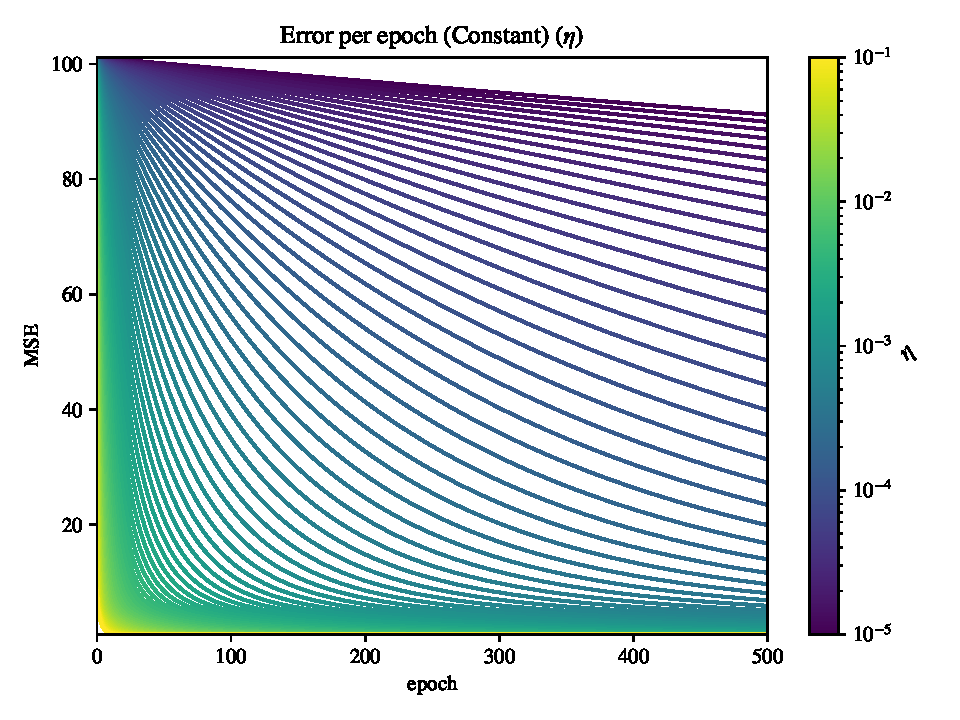
\includegraphics[width=5.5cm]{Project2/figures/polynomial_grad/OLS_analytic/constant_error.pdf} }}%
    \qquad
    \subfloat[\centering Automatic differentiation of OLS.]{{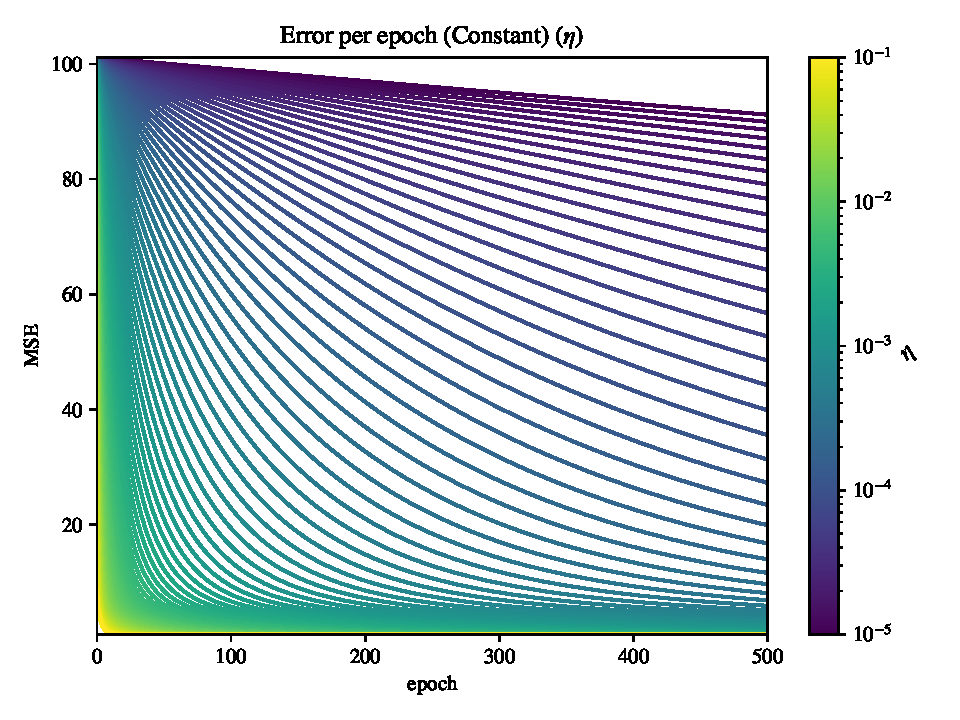
\includegraphics[width=5.5cm]{Project2/figures/polynomial_grad/OLS_autodiff/constant_error.pdf} }}%
    \caption{MSE of Gradient Descent with OLS over epochs for varying values of $\eta$.}%
    \label{fig:GDconstanterror}%
\end{figure}

As we see in \autoref{fig:GDconstanttheta} and \autoref{fig:GDconstanterror}, we get identical results using automatic differentiation and the analytical expression. We found the same results across the board, and the results using the analytic expressions will therefore be excluded from this section for the sake of brevity. In \autoref{fig:GDconstantpred} we see how Gradient Descent fits the target polynomial, predicting it almost perfectly for higher learning rates.

\begin{figure}[H]%
    \centering
    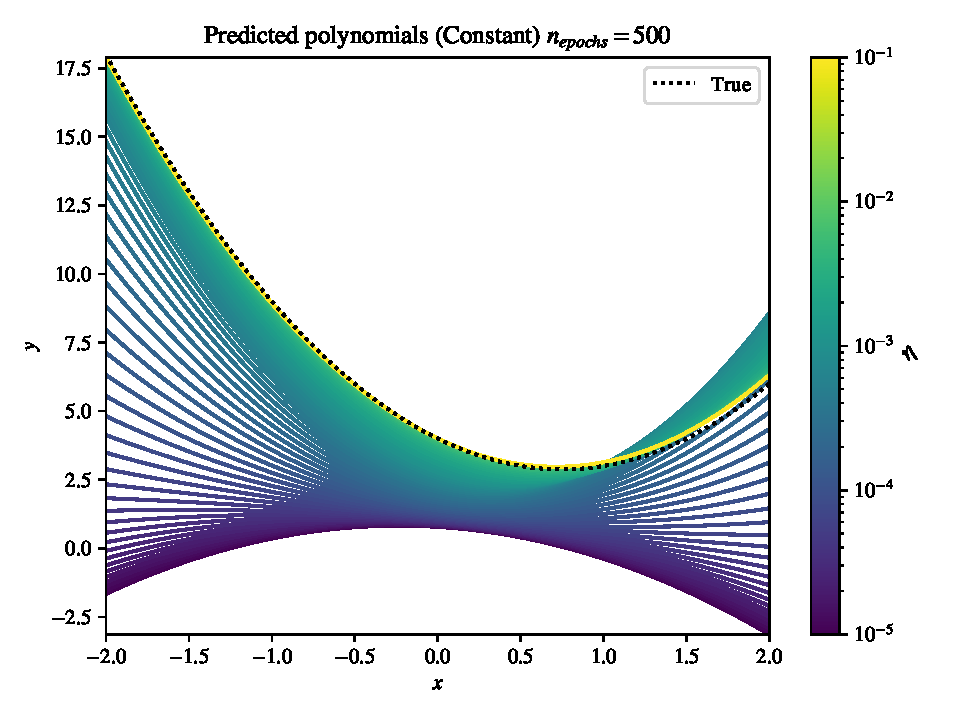
\includegraphics[width=8cm]{Project2/figures/polynomial_grad/OLS_autodiff/constant_prediction.pdf}
    \caption{Predicted polynomials for the resulting parameter values $\theta$ from Gradient descent with constant learning rate after 500 epochs.}
    \label{fig:GDconstantpred}
\end{figure}

Introducing momentum, as in (\ref{eq:momentum_eq}) to our model can greatly improve results. We begin by seeing how the behaviour in \autoref{fig:ZigZagMomentumGradientDescent} is seen in our case.

\begin{figure}[H]%
    \centering
    \subfloat[\centering Error for varying $\rho$.]{{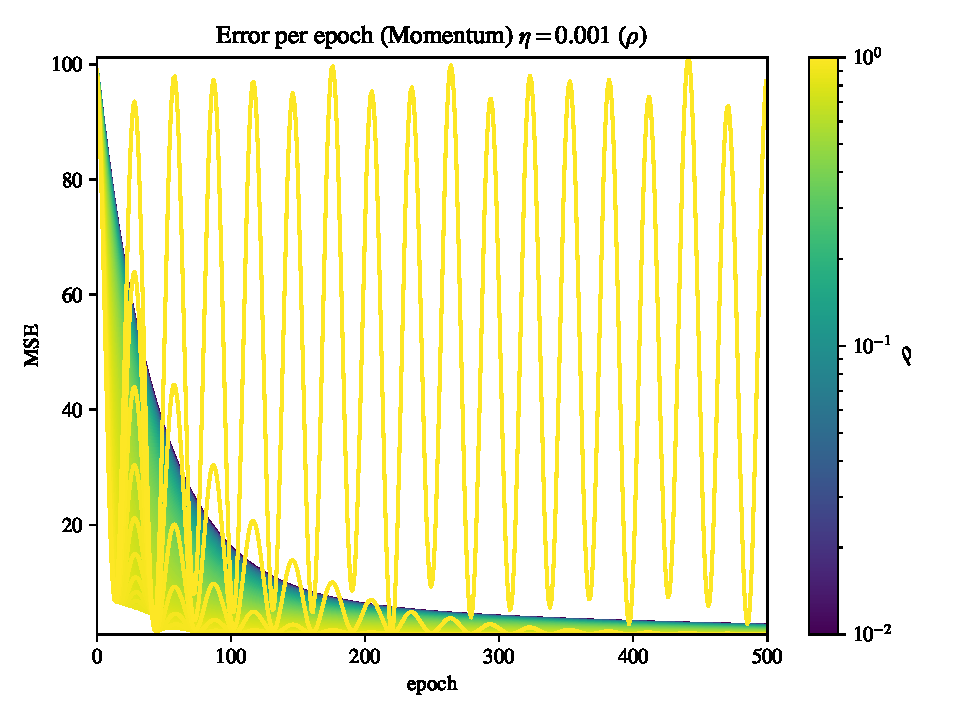
\includegraphics[width=5.5cm]{Project2/figures/polynomial_grad/OLS_analytic/momentum_error_rho.pdf} }}%
    \qquad
    \subfloat[\centering Parameters $\theta$ for varying $\rho$.]{{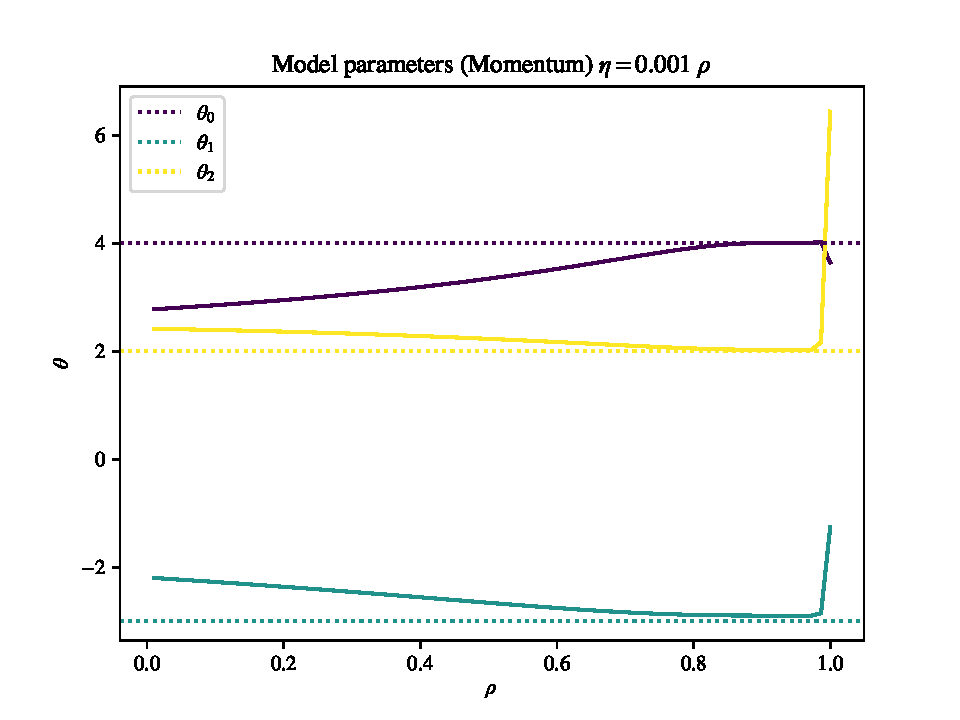
\includegraphics[width=5.5cm]{Project2/figures/polynomial_grad/OLS_autodiff/momentum_thetas_rho.pdf} }}%
    \caption{Gradient descent with varying momentum values $\rho$ over 500 epochs with a learning rate of $\eta = 10^{-3}$.}%
    \label{fig:GDmomentumrho}%
\end{figure}

As we see in \autoref{fig:GDmomentumrho}, we get greatly improved convergence results with higher values of $\rho$, although we have to be careful as we approach $\rho = 1$ as it can become quite unstable. Due to this, we settle for a value of $\rho = 0.9$ for the rest of our exploration.

\begin{figure}[H]%
    \centering
    \subfloat[\centering Error for varying $\eta$.]{{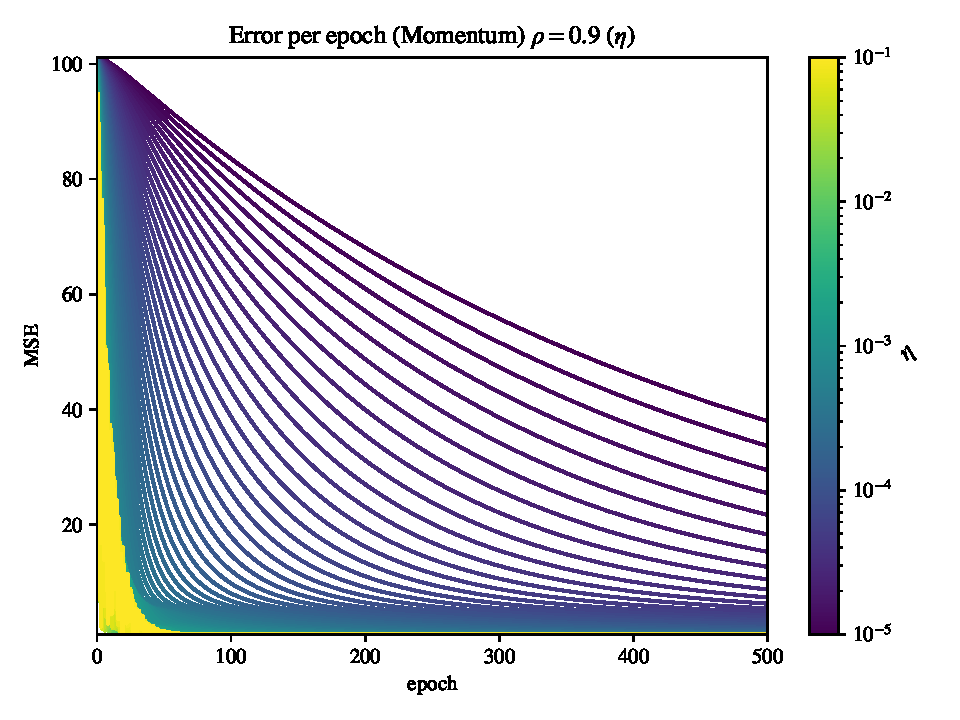
\includegraphics[width=5.5cm]{Project2/figures/polynomial_grad/OLS_analytic/momentum_error_eta.pdf} }}%
    \qquad
    \subfloat[\centering Parameters $\theta$ for varying $\eta$.]{{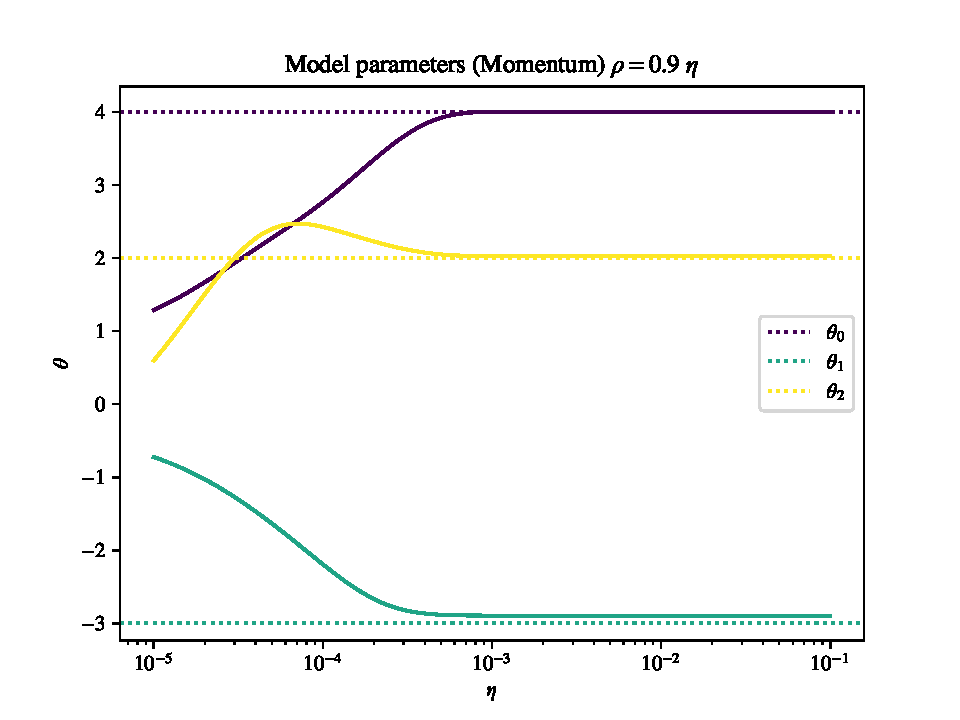
\includegraphics[width=5.5cm]{Project2/figures/polynomial_grad/OLS_autodiff/momentum_thetas_eta.pdf} }}%
    \caption{Gradient descent with momentum $\rho=0.9$ over 500 epochs with varying $\eta$.}%
    \label{fig:GDmomentumeta}%
\end{figure}

\begin{figure}[H]%
    \centering
    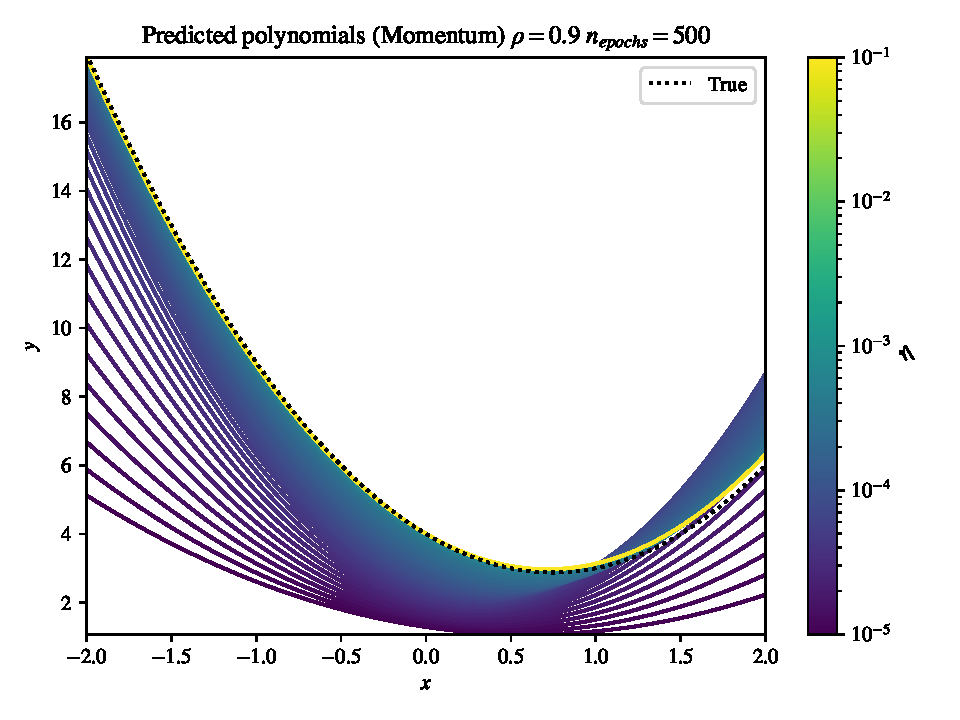
\includegraphics[width=8cm]{Project2/figures/polynomial_grad/OLS_autodiff/momentum_prediction_eta.pdf}
    \caption{Predicted polynomials for the resulting parameter values $\theta$ from Gradient descent with constant learning rate after 500 epochs.}
    \label{fig:GDmomentumpred}
\end{figure}

\newpage
\section{Discussion}

\section{Conclusion}

\section{References}

\printbibliography
% \bibliography{Project2/refs} % add  references to this 

\section{Appendix}
The code is publicly available on \href{https://github.com/augustfe/FYSSTK}{github.com/augustfe/FYSSTK}, written in python.


\end{document}